\documentclass[1p]{elsarticle_modified}
%\bibliographystyle{elsarticle-num}

%\usepackage[colorlinks]{hyperref}
%\usepackage{abbrmath_seonhwa} %\Abb, \Ascr, \Acal ,\Abf, \Afrak
\usepackage{amsfonts}
\usepackage{amssymb}
\usepackage{amsmath}
\usepackage{amsthm}
\usepackage{scalefnt}
\usepackage{amsbsy}
\usepackage{kotex}
\usepackage{caption}
\usepackage{subfig}
\usepackage{color}
\usepackage{graphicx}
\usepackage{xcolor} %% white, black, red, green, blue, cyan, magenta, yellow
\usepackage{float}
\usepackage{setspace}
\usepackage{hyperref}

\usepackage{tikz}
\usetikzlibrary{arrows}

\usepackage{multirow}
\usepackage{array} % fixed length table
\usepackage{hhline}

%%%%%%%%%%%%%%%%%%%%%
\makeatletter
\renewcommand*\env@matrix[1][\arraystretch]{%
	\edef\arraystretch{#1}%
	\hskip -\arraycolsep
	\let\@ifnextchar\new@ifnextchar
	\array{*\c@MaxMatrixCols c}}
\makeatother %https://tex.stackexchange.com/questions/14071/how-can-i-increase-the-line-spacing-in-a-matrix
%%%%%%%%%%%%%%%

\usepackage[normalem]{ulem}

\newcommand{\msout}[1]{\ifmmode\text{\sout{\ensuremath{#1}}}\else\sout{#1}\fi}
%SOURCE: \msout is \stkout macro in https://tex.stackexchange.com/questions/20609/strikeout-in-math-mode

\newcommand{\cancel}[1]{
	\ifmmode
	{\color{red}\msout{#1}}
	\else
	{\color{red}\sout{#1}}
	\fi
}

\newcommand{\add}[1]{
	{\color{blue}\uwave{#1}}
}

\newcommand{\replace}[2]{
	\ifmmode
	{\color{red}\msout{#1}}{\color{blue}\uwave{#2}}
	\else
	{\color{red}\sout{#1}}{\color{blue}\uwave{#2}}
	\fi
}

\newcommand{\Sol}{\mathcal{S}} %segment
\newcommand{\D}{D} %diagram
\newcommand{\A}{\mathcal{A}} %arc


%%%%%%%%%%%%%%%%%%%%%%%%%%%%%5 test

\def\sl{\operatorname{\textup{SL}}(2,\Cbb)}
\def\psl{\operatorname{\textup{PSL}}(2,\Cbb)}
\def\quan{\mkern 1mu \triangleright \mkern 1mu}

\theoremstyle{definition}
\newtheorem{thm}{Theorem}[section]
\newtheorem{prop}[thm]{Proposition}
\newtheorem{lem}[thm]{Lemma}
\newtheorem{ques}[thm]{Question}
\newtheorem{cor}[thm]{Corollary}
\newtheorem{defn}[thm]{Definition}
\newtheorem{exam}[thm]{Example}
\newtheorem{rmk}[thm]{Remark}
\newtheorem{alg}[thm]{Algorithm}

\newcommand{\I}{\sqrt{-1}}
\begin{document}

%\begin{frontmatter}
%
%\title{Boundary parabolic representations of knots up to 8 crossings}
%
%%% Group authors per affiliation:
%\author{Yunhi Cho} 
%\address{Department of Mathematics, University of Seoul, Seoul, Korea}
%\ead{yhcho@uos.ac.kr}
%
%
%\author{Seonhwa Kim} %\fnref{s_kim}}
%\address{Center for Geometry and Physics, Institute for Basic Science, Pohang, 37673, Korea}
%\ead{ryeona17@ibs.re.kr}
%
%\author{Hyuk Kim}
%\address{Department of Mathematical Sciences, Seoul National University, Seoul 08826, Korea}
%\ead{hyukkim@snu.ac.kr}
%
%\author{Seokbeom Yoon}
%\address{Department of Mathematical Sciences, Seoul National University, Seoul, 08826,  Korea}
%\ead{sbyoon15@snu.ac.kr}
%
%\begin{abstract}
%We find all boundary parabolic representation of knots up to 8 crossings.
%
%\end{abstract}
%\begin{keyword}
%    \MSC[2010] 57M25 
%\end{keyword}
%
%\end{frontmatter}

%\linenumbers
%\tableofcontents
%
\newcommand\colored[1]{\textcolor{white}{\rule[-0.35ex]{0.8em}{1.4ex}}\kern-0.8em\color{red} #1}%
%\newcommand\colored[1]{\textcolor{white}{ #1}\kern-2.17ex	\textcolor{white}{ #1}\kern-1.81ex	\textcolor{white}{ #1}\kern-2.15ex\color{red}#1	}

{\Large $\underline{12a_{0755}~(K12a_{0755})}$}

\setlength{\tabcolsep}{10pt}
\renewcommand{\arraystretch}{1.6}
\vspace{1cm}\begin{tabular}{m{100pt}>{\centering\arraybackslash}m{274pt}}
\multirow{5}{120pt}{
	\centering
	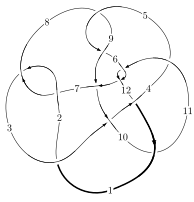
\includegraphics[width=112pt]{../../../GIT/diagram.site/Diagrams/png/1556_12a_0755.png}\\
\ \ \ A knot diagram\footnotemark}&
\allowdisplaybreaks
\textbf{Linearized knot diagam} \\
\cline{2-2}
 &
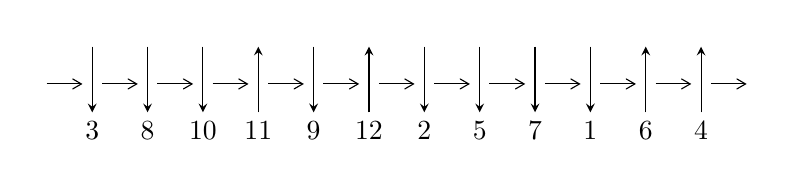
\begin{tikzpicture}[x=20pt, y=17pt]
	% nodes
	\node (C0) at (0, 0) {};
	\node (C1) at (1, 0) {};
	\node (C1U) at (1, +1) {};
	\node (C1D) at (1, -1) {3};

	\node (C2) at (2, 0) {};
	\node (C2U) at (2, +1) {};
	\node (C2D) at (2, -1) {8};

	\node (C3) at (3, 0) {};
	\node (C3U) at (3, +1) {};
	\node (C3D) at (3, -1) {10};

	\node (C4) at (4, 0) {};
	\node (C4U) at (4, +1) {};
	\node (C4D) at (4, -1) {11};

	\node (C5) at (5, 0) {};
	\node (C5U) at (5, +1) {};
	\node (C5D) at (5, -1) {9};

	\node (C6) at (6, 0) {};
	\node (C6U) at (6, +1) {};
	\node (C6D) at (6, -1) {12};

	\node (C7) at (7, 0) {};
	\node (C7U) at (7, +1) {};
	\node (C7D) at (7, -1) {2};

	\node (C8) at (8, 0) {};
	\node (C8U) at (8, +1) {};
	\node (C8D) at (8, -1) {5};

	\node (C9) at (9, 0) {};
	\node (C9U) at (9, +1) {};
	\node (C9D) at (9, -1) {7};

	\node (C10) at (10, 0) {};
	\node (C10U) at (10, +1) {};
	\node (C10D) at (10, -1) {1};

	\node (C11) at (11, 0) {};
	\node (C11U) at (11, +1) {};
	\node (C11D) at (11, -1) {6};

	\node (C12) at (12, 0) {};
	\node (C12U) at (12, +1) {};
	\node (C12D) at (12, -1) {4};
	\node (C13) at (13, 0) {};

	% arrows
	\draw[->,>={angle 60}]
	(C0) edge (C1) (C1) edge (C2) (C2) edge (C3) (C3) edge (C4) (C4) edge (C5) (C5) edge (C6) (C6) edge (C7) (C7) edge (C8) (C8) edge (C9) (C9) edge (C10) (C10) edge (C11) (C11) edge (C12) (C12) edge (C13) ;	\draw[->,>=stealth]
	(C1U) edge (C1D) (C2U) edge (C2D) (C3U) edge (C3D) (C4D) edge (C4U) (C5U) edge (C5D) (C6D) edge (C6U) (C7U) edge (C7D) (C8U) edge (C8D) (C9U) edge (C9D) (C10U) edge (C10D) (C11D) edge (C11U) (C12D) edge (C12U) ;
	\end{tikzpicture} \\
\hhline{~~} \\& 
\textbf{Solving Sequence} \\ \cline{2-2} 
 &
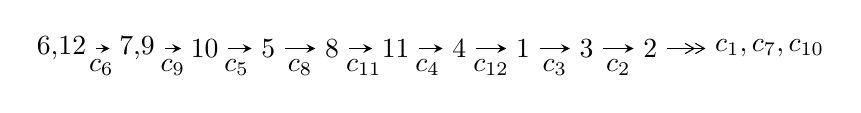
\begin{tikzpicture}[x=23pt, y=7pt]
	% node
	\node (A0) at (-1/8, 0) {6,12};
	\node (A1) at (17/16, 0) {7,9};
	\node (A2) at (17/8, 0) {10};
	\node (A3) at (25/8, 0) {5};
	\node (A4) at (33/8, 0) {8};
	\node (A5) at (41/8, 0) {11};
	\node (A6) at (49/8, 0) {4};
	\node (A7) at (57/8, 0) {1};
	\node (A8) at (65/8, 0) {3};
	\node (A9) at (73/8, 0) {2};
	\node (C1) at (1/2, -1) {$c_{6}$};
	\node (C2) at (13/8, -1) {$c_{9}$};
	\node (C3) at (21/8, -1) {$c_{5}$};
	\node (C4) at (29/8, -1) {$c_{8}$};
	\node (C5) at (37/8, -1) {$c_{11}$};
	\node (C6) at (45/8, -1) {$c_{4}$};
	\node (C7) at (53/8, -1) {$c_{12}$};
	\node (C8) at (61/8, -1) {$c_{3}$};
	\node (C9) at (69/8, -1) {$c_{2}$};
	\node (A10) at (11, 0) {$c_{1},c_{7},c_{10}$};

	% edge
	\draw[->,>=stealth]	
	(A0) edge (A1) (A1) edge (A2) (A2) edge (A3) (A3) edge (A4) (A4) edge (A5) (A5) edge (A6) (A6) edge (A7) (A7) edge (A8) (A8) edge (A9) ;
	\draw[->>,>={angle 60}]	
	(A9) edge (A10);
\end{tikzpicture} \\ 

\end{tabular} \\

\footnotetext{
The image of knot diagram is generated by the software ``\textbf{Draw programme}" developed by Andrew Bartholomew(\url{http://www.layer8.co.uk/maths/draw/index.htm\#Running-draw}), where we modified some parts for our purpose(\url{https://github.com/CATsTAILs/LinksPainter}).
}\phantom \\ \newline 
\centering \textbf{Ideals for irreducible components\footnotemark of $X_{\text{par}}$} 
 
\begin{align*}
I^u_{1}&=\langle 
6.46942\times10^{1040} u^{179}-2.62189\times10^{1042} u^{178}+\cdots+1.27215\times10^{1044} b-1.16593\times10^{1046},\\
\phantom{I^u_{1}}&\phantom{= \langle  }-8.30947\times10^{1047} u^{179}-2.59048\times10^{1047} u^{178}+\cdots+1.29887\times10^{1047} a+1.26957\times10^{1051},\\
\phantom{I^u_{1}}&\phantom{= \langle  }u^{180}+u^{179}+\cdots-758 u-1021\rangle \\
I^u_{2}&=\langle 
-1.16181\times10^{28} u^{44}+9.07809\times10^{27} u^{43}+\cdots+1.13258\times10^{27} b+2.27919\times10^{28},\\
\phantom{I^u_{2}}&\phantom{= \langle  }-1.18648\times10^{36} u^{44}+7.69318\times10^{35} u^{43}+\cdots+1.37485\times10^{34} a+1.64948\times10^{36},\\
\phantom{I^u_{2}}&\phantom{= \langle  }u^{45}-11 u^{43}+\cdots+2 u-1\rangle \\
\\
\end{align*}
\raggedright * 2 irreducible components of $\dim_{\mathbb{C}}=0$, with total 225 representations.\\
\footnotetext{All coefficients of polynomials are rational numbers. But the coefficients are sometimes approximated in decimal forms when there is not enough margin.}
\newpage
\renewcommand{\arraystretch}{1}
\centering \section*{I. $I^u_{1}= \langle 6.47\times10^{1040} u^{179}-2.62\times10^{1042} u^{178}+\cdots+1.27\times10^{1044} b-1.17\times10^{1046},\;-8.31\times10^{1047} u^{179}-2.59\times10^{1047} u^{178}+\cdots+1.30\times10^{1047} a+1.27\times10^{1051},\;u^{180}+u^{179}+\cdots-758 u-1021 \rangle$}
\flushleft \textbf{(i) Arc colorings}\\
\begin{tabular}{m{7pt} m{180pt} m{7pt} m{180pt} }
\flushright $a_{6}=$&$\begin{pmatrix}1\\0\end{pmatrix}$ \\
\flushright $a_{12}=$&$\begin{pmatrix}0\\u\end{pmatrix}$ \\
\flushright $a_{7}=$&$\begin{pmatrix}1\\- u^2\end{pmatrix}$ \\
\flushright $a_{9}=$&$\begin{pmatrix}6.39748 u^{179}+1.99441 u^{178}+\cdots+6979.93 u-9774.44\\-0.000508542 u^{179}+0.0206099 u^{178}+\cdots-28.9465 u+91.6505\end{pmatrix}$ \\
\flushright $a_{10}=$&$\begin{pmatrix}3.46652 u^{179}+1.06821 u^{178}+\cdots+3814.58 u-5370.56\\1.36513 u^{179}+0.454516 u^{178}+\cdots+1443.96 u-1955.21\end{pmatrix}$ \\
\flushright $a_{5}=$&$\begin{pmatrix}3.79544 u^{179}+1.22942 u^{178}+\cdots+4136.52 u-5632.08\\-0.148231 u^{179}-0.0220783 u^{178}+\cdots-66.4305 u+202.432\end{pmatrix}$ \\
\flushright $a_{8}=$&$\begin{pmatrix}4.21091 u^{179}+1.19632 u^{178}+\cdots+4437.64 u-6570.69\\0.00432269 u^{179}+0.135364 u^{178}+\cdots+176.418 u+164.437\end{pmatrix}$ \\
\flushright $a_{11}=$&$\begin{pmatrix}- u\\u\end{pmatrix}$ \\
\flushright $a_{4}=$&$\begin{pmatrix}2.11858 u^{179}+0.671018 u^{178}+\cdots+2262.14 u-3140.98\\1.52863 u^{179}+0.536325 u^{178}+\cdots+1807.95 u-2288.67\end{pmatrix}$ \\
\flushright $a_{1}=$&$\begin{pmatrix}-1.56079 u^{179}-0.442388 u^{178}+\cdots-1483.13 u+2315.85\\-0.300723 u^{179}-0.129530 u^{178}+\cdots-383.029 u+399.106\end{pmatrix}$ \\
\flushright $a_{3}=$&$\begin{pmatrix}-1.24373 u^{179}-0.490347 u^{178}+\cdots-1742.93 u+1977.89\\-0.991737 u^{179}-0.256247 u^{178}+\cdots-952.526 u+1555.45\end{pmatrix}$ \\
\flushright $a_{2}=$&$\begin{pmatrix}3.27816 u^{179}+1.13776 u^{178}+\cdots+3613.16 u-4770.78\\-0.535606 u^{179}-0.257279 u^{178}+\cdots-689.852 u+718.550\end{pmatrix}$\\&\end{tabular}
\flushleft \textbf{(ii) Obstruction class $= -1$}\\~\\
\flushleft \textbf{(iii) Cusp Shapes $= -0.659722 u^{179}-0.371440 u^{178}+\cdots-607.760 u+665.189$}\\~\\
\newpage\renewcommand{\arraystretch}{1}
\flushleft \textbf{(iv) u-Polynomials at the component}\newline \\
\begin{tabular}{m{50pt}|m{274pt}}
Crossings & \hspace{64pt}u-Polynomials at each crossing \\
\hline $$\begin{aligned}c_{1}\end{aligned}$$&$\begin{aligned}
&u^{180}+71 u^{179}+\cdots+772300 u+22801
\end{aligned}$\\
\hline $$\begin{aligned}c_{2},c_{7}\end{aligned}$$&$\begin{aligned}
&u^{180}+u^{179}+\cdots-180 u-151
\end{aligned}$\\
\hline $$\begin{aligned}c_{3}\end{aligned}$$&$\begin{aligned}
&u^{180}+2 u^{179}+\cdots-45 u+1
\end{aligned}$\\
\hline $$\begin{aligned}c_{4}\end{aligned}$$&$\begin{aligned}
&u^{180}- u^{179}+\cdots+565923008 u-391286809
\end{aligned}$\\
\hline $$\begin{aligned}c_{5},c_{8}\end{aligned}$$&$\begin{aligned}
&u^{180}+2 u^{179}+\cdots+731401 u+82807
\end{aligned}$\\
\hline $$\begin{aligned}c_{6},c_{11}\end{aligned}$$&$\begin{aligned}
&u^{180}+u^{179}+\cdots-758 u-1021
\end{aligned}$\\
\hline $$\begin{aligned}c_{9}\end{aligned}$$&$\begin{aligned}
&u^{180}-5 u^{179}+\cdots-3167561 u-887597
\end{aligned}$\\
\hline $$\begin{aligned}c_{10}\end{aligned}$$&$\begin{aligned}
&u^{180}-14 u^{179}+\cdots-360019 u+18833
\end{aligned}$\\
\hline $$\begin{aligned}c_{12}\end{aligned}$$&$\begin{aligned}
&u^{180}+12 u^{179}+\cdots+305 u+25
\end{aligned}$\\
\hline
\end{tabular}\\~\\
\newpage\renewcommand{\arraystretch}{1}
\flushleft \textbf{(v) Riley Polynomials at the component}\newline \\
\begin{tabular}{m{50pt}|m{274pt}}
Crossings & \hspace{64pt}Riley Polynomials at each crossing \\
\hline $$\begin{aligned}c_{1}\end{aligned}$$&$\begin{aligned}
&y^{180}+69 y^{179}+\cdots+393405409088 y+519885601
\end{aligned}$\\
\hline $$\begin{aligned}c_{2},c_{7}\end{aligned}$$&$\begin{aligned}
&y^{180}-71 y^{179}+\cdots-772300 y+22801
\end{aligned}$\\
\hline $$\begin{aligned}c_{3}\end{aligned}$$&$\begin{aligned}
&y^{180}+26 y^{179}+\cdots-13 y+1
\end{aligned}$\\
\hline $$\begin{aligned}c_{4}\end{aligned}$$&$\begin{aligned}
&y^{180}-17 y^{179}+\cdots-768200127417898812 y+153105366897402481
\end{aligned}$\\
\hline $$\begin{aligned}c_{5},c_{8}\end{aligned}$$&$\begin{aligned}
&y^{180}-90 y^{179}+\cdots-186489273469 y+6856999249
\end{aligned}$\\
\hline $$\begin{aligned}c_{6},c_{11}\end{aligned}$$&$\begin{aligned}
&y^{180}-95 y^{179}+\cdots-38394446 y+1042441
\end{aligned}$\\
\hline $$\begin{aligned}c_{9}\end{aligned}$$&$\begin{aligned}
&y^{180}+y^{179}+\cdots-19198314861057 y+787828434409
\end{aligned}$\\
\hline $$\begin{aligned}c_{10}\end{aligned}$$&$\begin{aligned}
&y^{180}+30 y^{179}+\cdots+35805184153 y+354681889
\end{aligned}$\\
\hline $$\begin{aligned}c_{12}\end{aligned}$$&$\begin{aligned}
&y^{180}+156 y^{178}+\cdots+35575 y+625
\end{aligned}$\\
\hline
\end{tabular}\\~\\
\newpage\flushleft \textbf{(vi) Complex Volumes and Cusp Shapes}
$$\begin{array}{c|c|c}  
\text{Solutions to }I^u_{1}& \I (\text{vol} + \sqrt{-1}CS) & \text{Cusp shape}\\
 \hline 
\begin{aligned}
u &= -0.544652 + 0.856933 I \\
a &= \phantom{-}0.353098 - 0.630739 I \\
b &= -0.888060 + 0.565610 I\end{aligned}
 & -2.18832 - 2.35646 I & \phantom{-0.000000 } 0 \\ \hline\begin{aligned}
u &= -0.544652 - 0.856933 I \\
a &= \phantom{-}0.353098 + 0.630739 I \\
b &= -0.888060 - 0.565610 I\end{aligned}
 & -2.18832 + 2.35646 I & \phantom{-0.000000 } 0 \\ \hline\begin{aligned}
u &= \phantom{-}0.858660 + 0.560485 I \\
a &= -1.10265 - 1.16702 I \\
b &= -0.617562 + 0.739902 I\end{aligned}
 & \phantom{-}3.46099 + 1.89790 I & \phantom{-0.000000 } 0 \\ \hline\begin{aligned}
u &= \phantom{-}0.858660 - 0.560485 I \\
a &= -1.10265 + 1.16702 I \\
b &= -0.617562 - 0.739902 I\end{aligned}
 & \phantom{-}3.46099 - 1.89790 I & \phantom{-0.000000 } 0 \\ \hline\begin{aligned}
u &= -0.967490 + 0.365847 I \\
a &= \phantom{-}1.08622 - 1.56153 I \\
b &= -0.37943 + 1.43434 I\end{aligned}
 & \phantom{-}4.66054 - 3.17592 I & \phantom{-0.000000 } 0 \\ \hline\begin{aligned}
u &= -0.967490 - 0.365847 I \\
a &= \phantom{-}1.08622 + 1.56153 I \\
b &= -0.37943 - 1.43434 I\end{aligned}
 & \phantom{-}4.66054 + 3.17592 I & \phantom{-0.000000 } 0 \\ \hline\begin{aligned}
u &= -0.861598 + 0.417149 I \\
a &= -0.05218 - 2.15259 I \\
b &= \phantom{-}0.934370 + 0.489622 I\end{aligned}
 & -1.54454 - 4.15543 I & \phantom{-0.000000 } 0 \\ \hline\begin{aligned}
u &= -0.861598 - 0.417149 I \\
a &= -0.05218 + 2.15259 I \\
b &= \phantom{-}0.934370 - 0.489622 I\end{aligned}
 & -1.54454 + 4.15543 I & \phantom{-0.000000 } 0 \\ \hline\begin{aligned}
u &= -0.962447 + 0.416308 I \\
a &= \phantom{-}0.77363 + 1.75507 I \\
b &= -1.200450 - 0.612984 I\end{aligned}
 & -5.53707 - 2.51693 I & \phantom{-0.000000 } 0 \\ \hline\begin{aligned}
u &= -0.962447 - 0.416308 I \\
a &= \phantom{-}0.77363 - 1.75507 I \\
b &= -1.200450 + 0.612984 I\end{aligned}
 & -5.53707 + 2.51693 I & \phantom{-0.000000 } 0\\
 \hline 
 \end{array}$$\newpage$$\begin{array}{c|c|c}  
\text{Solutions to }I^u_{1}& \I (\text{vol} + \sqrt{-1}CS) & \text{Cusp shape}\\
 \hline 
\begin{aligned}
u &= -0.999288 + 0.319199 I \\
a &= \phantom{-}0.818191 - 0.163003 I \\
b &= -0.744256 + 0.815866 I\end{aligned}
 & \phantom{-}3.08831 + 3.86688 I & \phantom{-0.000000 } 0 \\ \hline\begin{aligned}
u &= -0.999288 - 0.319199 I \\
a &= \phantom{-}0.818191 + 0.163003 I \\
b &= -0.744256 - 0.815866 I\end{aligned}
 & \phantom{-}3.08831 - 3.86688 I & \phantom{-0.000000 } 0 \\ \hline\begin{aligned}
u &= -0.771002 + 0.546425 I \\
a &= \phantom{-}0.47917 + 1.62861 I \\
b &= -1.335510 - 0.253643 I\end{aligned}
 & -4.16813 + 4.93589 I & \phantom{-0.000000 } 0 \\ \hline\begin{aligned}
u &= -0.771002 - 0.546425 I \\
a &= \phantom{-}0.47917 - 1.62861 I \\
b &= -1.335510 + 0.253643 I\end{aligned}
 & -4.16813 - 4.93589 I & \phantom{-0.000000 } 0 \\ \hline\begin{aligned}
u &= \phantom{-}1.046460 + 0.253603 I \\
a &= \phantom{-}0.57796 + 1.64382 I \\
b &= -0.63788 - 1.32819 I\end{aligned}
 & \phantom{-}4.34051 + 4.64779 I & \phantom{-0.000000 } 0 \\ \hline\begin{aligned}
u &= \phantom{-}1.046460 - 0.253603 I \\
a &= \phantom{-}0.57796 - 1.64382 I \\
b &= -0.63788 + 1.32819 I\end{aligned}
 & \phantom{-}4.34051 - 4.64779 I & \phantom{-0.000000 } 0 \\ \hline\begin{aligned}
u &= -1.026850 + 0.327802 I \\
a &= -0.61461 - 2.39323 I \\
b &= \phantom{-}1.131340 + 0.426064 I\end{aligned}
 & -0.65133 - 4.75263 I & \phantom{-0.000000 } 0 \\ \hline\begin{aligned}
u &= -1.026850 - 0.327802 I \\
a &= -0.61461 + 2.39323 I \\
b &= \phantom{-}1.131340 - 0.426064 I\end{aligned}
 & -0.65133 + 4.75263 I & \phantom{-0.000000 } 0 \\ \hline\begin{aligned}
u &= -0.399718 + 1.008750 I \\
a &= -0.436601 - 0.225868 I \\
b &= -0.960412 + 0.350083 I\end{aligned}
 & -2.21102 + 1.15028 I & \phantom{-0.000000 } 0 \\ \hline\begin{aligned}
u &= -0.399718 - 1.008750 I \\
a &= -0.436601 + 0.225868 I \\
b &= -0.960412 - 0.350083 I\end{aligned}
 & -2.21102 - 1.15028 I & \phantom{-0.000000 } 0\\
 \hline 
 \end{array}$$\newpage$$\begin{array}{c|c|c}  
\text{Solutions to }I^u_{1}& \I (\text{vol} + \sqrt{-1}CS) & \text{Cusp shape}\\
 \hline 
\begin{aligned}
u &= \phantom{-}1.030690 + 0.346978 I \\
a &= -1.11250 - 1.40448 I \\
b &= \phantom{-}0.47107 + 1.33545 I\end{aligned}
 & \phantom{-}4.71254 - 1.28878 I & \phantom{-0.000000 } 0 \\ \hline\begin{aligned}
u &= \phantom{-}1.030690 - 0.346978 I \\
a &= -1.11250 + 1.40448 I \\
b &= \phantom{-}0.47107 - 1.33545 I\end{aligned}
 & \phantom{-}4.71254 + 1.28878 I & \phantom{-0.000000 } 0 \\ \hline\begin{aligned}
u &= -0.795351 + 0.439349 I \\
a &= -0.394551 - 0.558444 I \\
b &= \phantom{-}1.60867 + 0.01926 I\end{aligned}
 & -4.15704 - 8.98961 I & \phantom{-0.000000 } 0 \\ \hline\begin{aligned}
u &= -0.795351 - 0.439349 I \\
a &= -0.394551 + 0.558444 I \\
b &= \phantom{-}1.60867 - 0.01926 I\end{aligned}
 & -4.15704 + 8.98961 I & \phantom{-0.000000 } 0 \\ \hline\begin{aligned}
u &= \phantom{-}0.658525 + 0.876293 I \\
a &= -0.448538 - 0.461235 I \\
b &= \phantom{-}1.077040 + 0.527167 I\end{aligned}
 & -2.49064 - 1.62266 I & \phantom{-0.000000 } 0 \\ \hline\begin{aligned}
u &= \phantom{-}0.658525 - 0.876293 I \\
a &= -0.448538 + 0.461235 I \\
b &= \phantom{-}1.077040 - 0.527167 I\end{aligned}
 & -2.49064 + 1.62266 I & \phantom{-0.000000 } 0 \\ \hline\begin{aligned}
u &= \phantom{-}1.057840 + 0.305101 I \\
a &= -0.914371 - 0.505553 I \\
b &= \phantom{-}0.653215 + 0.860470 I\end{aligned}
 & \phantom{-}3.72825 + 1.22255 I & \phantom{-0.000000 } 0 \\ \hline\begin{aligned}
u &= \phantom{-}1.057840 - 0.305101 I \\
a &= -0.914371 + 0.505553 I \\
b &= \phantom{-}0.653215 - 0.860470 I\end{aligned}
 & \phantom{-}3.72825 - 1.22255 I & \phantom{-0.000000 } 0 \\ \hline\begin{aligned}
u &= -0.706400 + 0.555166 I \\
a &= -0.144991 - 0.084069 I \\
b &= -1.015630 + 0.190671 I\end{aligned}
 & -1.82917 + 0.21089 I & \phantom{-0.000000 } 0 \\ \hline\begin{aligned}
u &= -0.706400 - 0.555166 I \\
a &= -0.144991 + 0.084069 I \\
b &= -1.015630 - 0.190671 I\end{aligned}
 & -1.82917 - 0.21089 I & \phantom{-0.000000 } 0\\
 \hline 
 \end{array}$$\newpage$$\begin{array}{c|c|c}  
\text{Solutions to }I^u_{1}& \I (\text{vol} + \sqrt{-1}CS) & \text{Cusp shape}\\
 \hline 
\begin{aligned}
u &= \phantom{-}0.833701 + 0.323163 I \\
a &= \phantom{-}0.115274 - 0.219384 I \\
b &= -1.46859 - 0.07425 I\end{aligned}
 & -1.61760 + 4.01420 I & \phantom{-0.000000 } 0 \\ \hline\begin{aligned}
u &= \phantom{-}0.833701 - 0.323163 I \\
a &= \phantom{-}0.115274 + 0.219384 I \\
b &= -1.46859 + 0.07425 I\end{aligned}
 & -1.61760 - 4.01420 I & \phantom{-0.000000 } 0 \\ \hline\begin{aligned}
u &= \phantom{-}0.134108 + 0.883852 I \\
a &= \phantom{-}0.164549 - 0.118172 I \\
b &= \phantom{-}1.165680 - 0.403607 I\end{aligned}
 & -1.93976 + 7.29622 I & \phantom{-0.000000 } 0 \\ \hline\begin{aligned}
u &= \phantom{-}0.134108 - 0.883852 I \\
a &= \phantom{-}0.164549 + 0.118172 I \\
b &= \phantom{-}1.165680 + 0.403607 I\end{aligned}
 & -1.93976 - 7.29622 I & \phantom{-0.000000 } 0 \\ \hline\begin{aligned}
u &= -0.954125 + 0.564822 I \\
a &= \phantom{-}0.94446 - 1.44653 I \\
b &= \phantom{-}0.769698 + 0.802098 I\end{aligned}
 & \phantom{-}3.39181 - 7.30281 I & \phantom{-0.000000 } 0 \\ \hline\begin{aligned}
u &= -0.954125 - 0.564822 I \\
a &= \phantom{-}0.94446 + 1.44653 I \\
b &= \phantom{-}0.769698 - 0.802098 I\end{aligned}
 & \phantom{-}3.39181 + 7.30281 I & \phantom{-0.000000 } 0 \\ \hline\begin{aligned}
u &= \phantom{-}0.818772 + 0.749291 I \\
a &= -0.326308 - 0.060149 I \\
b &= \phantom{-}1.181920 + 0.251409 I\end{aligned}
 & -2.81671 + 3.20015 I & \phantom{-0.000000 } 0 \\ \hline\begin{aligned}
u &= \phantom{-}0.818772 - 0.749291 I \\
a &= -0.326308 + 0.060149 I \\
b &= \phantom{-}1.181920 - 0.251409 I\end{aligned}
 & -2.81671 - 3.20015 I & \phantom{-0.000000 } 0 \\ \hline\begin{aligned}
u &= \phantom{-}0.816264 + 0.754277 I \\
a &= -0.10381 - 1.79852 I \\
b &= -0.897029 + 0.748328 I\end{aligned}
 & -2.01951 + 7.53940 I & \phantom{-0.000000 } 0 \\ \hline\begin{aligned}
u &= \phantom{-}0.816264 - 0.754277 I \\
a &= -0.10381 + 1.79852 I \\
b &= -0.897029 - 0.748328 I\end{aligned}
 & -2.01951 - 7.53940 I & \phantom{-0.000000 } 0\\
 \hline 
 \end{array}$$\newpage$$\begin{array}{c|c|c}  
\text{Solutions to }I^u_{1}& \I (\text{vol} + \sqrt{-1}CS) & \text{Cusp shape}\\
 \hline 
\begin{aligned}
u &= -0.896847 + 0.662839 I \\
a &= \phantom{-}0.08115 - 1.84945 I \\
b &= \phantom{-}0.759907 + 0.677854 I\end{aligned}
 & -1.18795 - 3.20557 I & \phantom{-0.000000 } 0 \\ \hline\begin{aligned}
u &= -0.896847 - 0.662839 I \\
a &= \phantom{-}0.08115 + 1.84945 I \\
b &= \phantom{-}0.759907 - 0.677854 I\end{aligned}
 & -1.18795 + 3.20557 I & \phantom{-0.000000 } 0 \\ \hline\begin{aligned}
u &= -0.950258 + 0.590530 I \\
a &= \phantom{-}0.21391 - 1.39805 I \\
b &= \phantom{-}0.616278 - 0.028724 I\end{aligned}
 & \phantom{-}0.87027 - 4.86559 I & \phantom{-0.000000 } 0 \\ \hline\begin{aligned}
u &= -0.950258 - 0.590530 I \\
a &= \phantom{-}0.21391 + 1.39805 I \\
b &= \phantom{-}0.616278 + 0.028724 I\end{aligned}
 & \phantom{-}0.87027 + 4.86559 I & \phantom{-0.000000 } 0 \\ \hline\begin{aligned}
u &= \phantom{-}1.073410 + 0.330573 I \\
a &= \phantom{-}0.88043 - 2.36486 I \\
b &= -1.211100 + 0.381137 I\end{aligned}
 & -1.87778 + 9.84922 I & \phantom{-0.000000 } 0 \\ \hline\begin{aligned}
u &= \phantom{-}1.073410 - 0.330573 I \\
a &= \phantom{-}0.88043 + 2.36486 I \\
b &= -1.211100 - 0.381137 I\end{aligned}
 & -1.87778 - 9.84922 I & \phantom{-0.000000 } 0 \\ \hline\begin{aligned}
u &= \phantom{-}0.799901 + 0.349974 I \\
a &= -0.63357 + 2.05521 I \\
b &= \phantom{-}1.032160 - 0.358952 I\end{aligned}
 & -1.66606 - 0.94848 I & \phantom{-0.000000 } 0 \\ \hline\begin{aligned}
u &= \phantom{-}0.799901 - 0.349974 I \\
a &= -0.63357 - 2.05521 I \\
b &= \phantom{-}1.032160 + 0.358952 I\end{aligned}
 & -1.66606 + 0.94848 I & \phantom{-0.000000 } 0 \\ \hline\begin{aligned}
u &= -0.871293 + 0.026419 I \\
a &= \phantom{-}0.38721 - 2.30721 I \\
b &= \phantom{-}1.007110 + 0.564764 I\end{aligned}
 & \phantom{-}2.41709 - 4.96606 I & \phantom{-0.000000 } 0 \\ \hline\begin{aligned}
u &= -0.871293 - 0.026419 I \\
a &= \phantom{-}0.38721 + 2.30721 I \\
b &= \phantom{-}1.007110 - 0.564764 I\end{aligned}
 & \phantom{-}2.41709 + 4.96606 I & \phantom{-0.000000 } 0\\
 \hline 
 \end{array}$$\newpage$$\begin{array}{c|c|c}  
\text{Solutions to }I^u_{1}& \I (\text{vol} + \sqrt{-1}CS) & \text{Cusp shape}\\
 \hline 
\begin{aligned}
u &= \phantom{-}0.866358 + 0.051079 I \\
a &= -0.44172 + 1.85510 I \\
b &= -1.062440 - 0.517302 I\end{aligned}
 & \phantom{-}2.58754 + 0.87376 I & \phantom{-0.000000 } 0 \\ \hline\begin{aligned}
u &= \phantom{-}0.866358 - 0.051079 I \\
a &= -0.44172 - 1.85510 I \\
b &= -1.062440 + 0.517302 I\end{aligned}
 & \phantom{-}2.58754 - 0.87376 I & \phantom{-0.000000 } 0 \\ \hline\begin{aligned}
u &= -0.817214 + 0.235498 I \\
a &= \phantom{-}0.84699 - 1.81913 I \\
b &= -0.126436 + 1.407170 I\end{aligned}
 & \phantom{-}3.88389 + 0.48967 I & \phantom{-0.000000 } 0 \\ \hline\begin{aligned}
u &= -0.817214 - 0.235498 I \\
a &= \phantom{-}0.84699 + 1.81913 I \\
b &= -0.126436 - 1.407170 I\end{aligned}
 & \phantom{-}3.88389 - 0.48967 I & \phantom{-0.000000 } 0 \\ \hline\begin{aligned}
u &= \phantom{-}0.452247 + 0.717887 I \\
a &= -0.56557 - 1.55660 I \\
b &= -1.029210 + 0.547501 I\end{aligned}
 & -3.64638 + 2.31168 I & \phantom{-0.000000 } 0 \\ \hline\begin{aligned}
u &= \phantom{-}0.452247 - 0.717887 I \\
a &= -0.56557 + 1.55660 I \\
b &= -1.029210 - 0.547501 I\end{aligned}
 & -3.64638 - 2.31168 I & \phantom{-0.000000 } 0 \\ \hline\begin{aligned}
u &= \phantom{-}0.837829 + 0.023977 I \\
a &= -0.33714 + 1.98624 I \\
b &= \phantom{-}0.004273 - 1.379410 I\end{aligned}
 & \phantom{-}3.04547 - 3.16514 I & \phantom{-0.000000 } 0 \\ \hline\begin{aligned}
u &= \phantom{-}0.837829 - 0.023977 I \\
a &= -0.33714 - 1.98624 I \\
b &= \phantom{-}0.004273 + 1.379410 I\end{aligned}
 & \phantom{-}3.04547 + 3.16514 I & \phantom{-0.000000 } 0 \\ \hline\begin{aligned}
u &= -1.149680 + 0.182280 I \\
a &= -0.38001 + 1.36524 I \\
b &= \phantom{-}0.518344 - 1.114800 I\end{aligned}
 & \phantom{-}6.63013 + 0.67239 I & \phantom{-0.000000 } 0 \\ \hline\begin{aligned}
u &= -1.149680 - 0.182280 I \\
a &= -0.38001 - 1.36524 I \\
b &= \phantom{-}0.518344 + 1.114800 I\end{aligned}
 & \phantom{-}6.63013 - 0.67239 I & \phantom{-0.000000 } 0\\
 \hline 
 \end{array}$$\newpage$$\begin{array}{c|c|c}  
\text{Solutions to }I^u_{1}& \I (\text{vol} + \sqrt{-1}CS) & \text{Cusp shape}\\
 \hline 
\begin{aligned}
u &= \phantom{-}1.085510 + 0.436676 I \\
a &= \phantom{-}0.74637 - 1.77078 I \\
b &= -1.084240 + 0.185420 I\end{aligned}
 & -5.28456 + 3.73767 I & \phantom{-0.000000 } 0 \\ \hline\begin{aligned}
u &= \phantom{-}1.085510 - 0.436676 I \\
a &= \phantom{-}0.74637 + 1.77078 I \\
b &= -1.084240 - 0.185420 I\end{aligned}
 & -5.28456 - 3.73767 I & \phantom{-0.000000 } 0 \\ \hline\begin{aligned}
u &= \phantom{-}1.161710 + 0.140485 I \\
a &= -1.031520 + 0.868086 I \\
b &= \phantom{-}0.541593 - 0.640642 I\end{aligned}
 & \phantom{-}3.78976 - 0.23686 I & \phantom{-0.000000 } 0 \\ \hline\begin{aligned}
u &= \phantom{-}1.161710 - 0.140485 I \\
a &= -1.031520 - 0.868086 I \\
b &= \phantom{-}0.541593 + 0.640642 I\end{aligned}
 & \phantom{-}3.78976 + 0.23686 I & \phantom{-0.000000 } 0 \\ \hline\begin{aligned}
u &= \phantom{-}1.060510 + 0.504574 I \\
a &= -0.04254 - 1.42720 I \\
b &= -1.39658 + 0.48115 I\end{aligned}
 & -1.08030 + 6.00401 I & \phantom{-0.000000 } 0 \\ \hline\begin{aligned}
u &= \phantom{-}1.060510 - 0.504574 I \\
a &= -0.04254 + 1.42720 I \\
b &= -1.39658 - 0.48115 I\end{aligned}
 & -1.08030 - 6.00401 I & \phantom{-0.000000 } 0 \\ \hline\begin{aligned}
u &= \phantom{-}1.138050 + 0.293481 I \\
a &= -1.01517 - 1.59294 I \\
b &= -1.002130 + 0.289534 I\end{aligned}
 & \phantom{-}3.75272 + 3.81024 I & \phantom{-0.000000 } 0 \\ \hline\begin{aligned}
u &= \phantom{-}1.138050 - 0.293481 I \\
a &= -1.01517 + 1.59294 I \\
b &= -1.002130 - 0.289534 I\end{aligned}
 & \phantom{-}3.75272 - 3.81024 I & \phantom{-0.000000 } 0 \\ \hline\begin{aligned}
u &= \phantom{-}0.364225 + 0.738569 I \\
a &= \phantom{-}0.162662 + 0.332479 I \\
b &= \phantom{-}1.278100 + 0.526116 I\end{aligned}
 & -0.98972 - 5.96088 I & \phantom{-0.000000 } 0 \\ \hline\begin{aligned}
u &= \phantom{-}0.364225 - 0.738569 I \\
a &= \phantom{-}0.162662 - 0.332479 I \\
b &= \phantom{-}1.278100 - 0.526116 I\end{aligned}
 & -0.98972 + 5.96088 I & \phantom{-0.000000 } 0\\
 \hline 
 \end{array}$$\newpage$$\begin{array}{c|c|c}  
\text{Solutions to }I^u_{1}& \I (\text{vol} + \sqrt{-1}CS) & \text{Cusp shape}\\
 \hline 
\begin{aligned}
u &= -0.065475 + 0.809888 I \\
a &= -0.976716 + 0.453899 I \\
b &= -0.278519 - 0.709195 I\end{aligned}
 & \phantom{-}2.17617 + 3.58604 I & \phantom{-0.000000 } 0 \\ \hline\begin{aligned}
u &= -0.065475 - 0.809888 I \\
a &= -0.976716 - 0.453899 I \\
b &= -0.278519 + 0.709195 I\end{aligned}
 & \phantom{-}2.17617 - 3.58604 I & \phantom{-0.000000 } 0 \\ \hline\begin{aligned}
u &= \phantom{-}0.150530 + 0.793266 I \\
a &= \phantom{-}1.056400 + 0.708005 I \\
b &= \phantom{-}0.176530 - 0.865905 I\end{aligned}
 & \phantom{-}0.72737 - 9.16943 I & \phantom{-0.000000 } 0 \\ \hline\begin{aligned}
u &= \phantom{-}0.150530 - 0.793266 I \\
a &= \phantom{-}1.056400 - 0.708005 I \\
b &= \phantom{-}0.176530 + 0.865905 I\end{aligned}
 & \phantom{-}0.72737 + 9.16943 I & \phantom{-0.000000 } 0 \\ \hline\begin{aligned}
u &= \phantom{-}0.520582 + 0.609539 I \\
a &= \phantom{-}0.104515 + 1.156690 I \\
b &= \phantom{-}1.289700 + 0.149462 I\end{aligned}
 & -2.75317 - 1.62014 I & \phantom{-0.000000 } 0 \\ \hline\begin{aligned}
u &= \phantom{-}0.520582 - 0.609539 I \\
a &= \phantom{-}0.104515 - 1.156690 I \\
b &= \phantom{-}1.289700 - 0.149462 I\end{aligned}
 & -2.75317 + 1.62014 I & \phantom{-0.000000 } 0 \\ \hline\begin{aligned}
u &= \phantom{-}0.331232 + 1.159550 I \\
a &= -0.224162 + 0.183102 I \\
b &= -1.126710 - 0.527863 I\end{aligned}
 & -0.28241 - 8.29945 I & \phantom{-0.000000 } 0 \\ \hline\begin{aligned}
u &= \phantom{-}0.331232 - 1.159550 I \\
a &= -0.224162 - 0.183102 I \\
b &= -1.126710 + 0.527863 I\end{aligned}
 & -0.28241 + 8.29945 I & \phantom{-0.000000 } 0 \\ \hline\begin{aligned}
u &= -1.120790 + 0.459988 I \\
a &= \phantom{-}0.117282 - 0.686946 I \\
b &= -0.509589 + 0.541882 I\end{aligned}
 & -1.138300 - 0.793069 I & \phantom{-0.000000 } 0 \\ \hline\begin{aligned}
u &= -1.120790 - 0.459988 I \\
a &= \phantom{-}0.117282 + 0.686946 I \\
b &= -0.509589 - 0.541882 I\end{aligned}
 & -1.138300 + 0.793069 I & \phantom{-0.000000 } 0\\
 \hline 
 \end{array}$$\newpage$$\begin{array}{c|c|c}  
\text{Solutions to }I^u_{1}& \I (\text{vol} + \sqrt{-1}CS) & \text{Cusp shape}\\
 \hline 
\begin{aligned}
u &= -0.324228 + 0.711456 I \\
a &= -0.347251 + 0.170590 I \\
b &= -1.123800 + 0.568451 I\end{aligned}
 & -0.323740 + 1.330340 I & \phantom{-0.000000 } 0 \\ \hline\begin{aligned}
u &= -0.324228 - 0.711456 I \\
a &= -0.347251 - 0.170590 I \\
b &= -1.123800 - 0.568451 I\end{aligned}
 & -0.323740 - 1.330340 I & \phantom{-0.000000 } 0 \\ \hline\begin{aligned}
u &= -0.294571 + 1.183130 I \\
a &= \phantom{-}0.139200 + 0.241626 I \\
b &= \phantom{-}1.197000 - 0.555546 I\end{aligned}
 & -2.2759 + 14.3484 I & \phantom{-0.000000 } 0 \\ \hline\begin{aligned}
u &= -0.294571 - 1.183130 I \\
a &= \phantom{-}0.139200 - 0.241626 I \\
b &= \phantom{-}1.197000 + 0.555546 I\end{aligned}
 & -2.2759 - 14.3484 I & \phantom{-0.000000 } 0 \\ \hline\begin{aligned}
u &= \phantom{-}1.140550 + 0.433144 I \\
a &= \phantom{-}0.226578 + 1.274700 I \\
b &= -0.102636 - 1.152640 I\end{aligned}
 & -0.74537 + 6.46765 I & \phantom{-0.000000 } 0 \\ \hline\begin{aligned}
u &= \phantom{-}1.140550 - 0.433144 I \\
a &= \phantom{-}0.226578 - 1.274700 I \\
b &= -0.102636 + 1.152640 I\end{aligned}
 & -0.74537 - 6.46765 I & \phantom{-0.000000 } 0 \\ \hline\begin{aligned}
u &= -0.147509 + 0.756671 I \\
a &= \phantom{-}0.164754 - 0.749718 I \\
b &= -0.196299 + 0.593717 I\end{aligned}
 & -1.55919 + 1.87982 I & \phantom{-0.000000 } 0 \\ \hline\begin{aligned}
u &= -0.147509 - 0.756671 I \\
a &= \phantom{-}0.164754 + 0.749718 I \\
b &= -0.196299 - 0.593717 I\end{aligned}
 & -1.55919 - 1.87982 I & \phantom{-0.000000 } 0 \\ \hline\begin{aligned}
u &= -1.192050 + 0.308145 I \\
a &= \phantom{-}0.80750 - 1.88074 I \\
b &= \phantom{-}0.977319 + 0.384239 I\end{aligned}
 & \phantom{-}3.52201 - 9.19808 I & \phantom{-0.000000 } 0 \\ \hline\begin{aligned}
u &= -1.192050 - 0.308145 I \\
a &= \phantom{-}0.80750 + 1.88074 I \\
b &= \phantom{-}0.977319 - 0.384239 I\end{aligned}
 & \phantom{-}3.52201 + 9.19808 I & \phantom{-0.000000 } 0\\
 \hline 
 \end{array}$$\newpage$$\begin{array}{c|c|c}  
\text{Solutions to }I^u_{1}& \I (\text{vol} + \sqrt{-1}CS) & \text{Cusp shape}\\
 \hline 
\begin{aligned}
u &= \phantom{-}1.108610 + 0.555508 I \\
a &= -0.00822 - 1.82667 I \\
b &= -1.39725 + 0.76974 I\end{aligned}
 & \phantom{-}1.21209 + 10.86510 I & \phantom{-0.000000 } 0 \\ \hline\begin{aligned}
u &= \phantom{-}1.108610 - 0.555508 I \\
a &= -0.00822 + 1.82667 I \\
b &= -1.39725 - 0.76974 I\end{aligned}
 & \phantom{-}1.21209 - 10.86510 I & \phantom{-0.000000 } 0 \\ \hline\begin{aligned}
u &= -1.113840 + 0.547780 I \\
a &= \phantom{-}0.17282 - 1.84492 I \\
b &= \phantom{-}1.28147 + 0.79434 I\end{aligned}
 & \phantom{-}1.96870 - 6.13886 I & \phantom{-0.000000 } 0 \\ \hline\begin{aligned}
u &= -1.113840 - 0.547780 I \\
a &= \phantom{-}0.17282 + 1.84492 I \\
b &= \phantom{-}1.28147 - 0.79434 I\end{aligned}
 & \phantom{-}1.96870 + 6.13886 I & \phantom{-0.000000 } 0 \\ \hline\begin{aligned}
u &= -0.049100 + 1.246410 I \\
a &= \phantom{-}0.331163 - 0.515682 I \\
b &= \phantom{-}1.073800 + 0.288692 I\end{aligned}
 & -5.24445 - 4.67701 I & \phantom{-0.000000 } 0 \\ \hline\begin{aligned}
u &= -0.049100 - 1.246410 I \\
a &= \phantom{-}0.331163 + 0.515682 I \\
b &= \phantom{-}1.073800 - 0.288692 I\end{aligned}
 & -5.24445 + 4.67701 I & \phantom{-0.000000 } 0 \\ \hline\begin{aligned}
u &= \phantom{-}1.218860 + 0.285883 I \\
a &= -0.619445 - 0.951208 I \\
b &= \phantom{-}0.351749 + 0.764126 I\end{aligned}
 & \phantom{-}2.80158 + 1.74662 I & \phantom{-0.000000 } 0 \\ \hline\begin{aligned}
u &= \phantom{-}1.218860 - 0.285883 I \\
a &= -0.619445 + 0.951208 I \\
b &= \phantom{-}0.351749 - 0.764126 I\end{aligned}
 & \phantom{-}2.80158 - 1.74662 I & \phantom{-0.000000 } 0 \\ \hline\begin{aligned}
u &= -0.713504 + 0.190350 I \\
a &= -0.836589 + 0.243306 I \\
b &= \phantom{-}1.67967 - 0.27177 I\end{aligned}
 & -6.73735 - 0.46894 I & \phantom{-0.000000 } 0 \\ \hline\begin{aligned}
u &= -0.713504 - 0.190350 I \\
a &= -0.836589 - 0.243306 I \\
b &= \phantom{-}1.67967 + 0.27177 I\end{aligned}
 & -6.73735 + 0.46894 I & \phantom{-0.000000 } 0\\
 \hline 
 \end{array}$$\newpage$$\begin{array}{c|c|c}  
\text{Solutions to }I^u_{1}& \I (\text{vol} + \sqrt{-1}CS) & \text{Cusp shape}\\
 \hline 
\begin{aligned}
u &= \phantom{-}1.226170 + 0.361886 I \\
a &= -0.579858 - 1.011020 I \\
b &= \phantom{-}0.394373 + 0.753679 I\end{aligned}
 & \phantom{-}2.78506 + 1.79914 I & \phantom{-0.000000 } 0 \\ \hline\begin{aligned}
u &= \phantom{-}1.226170 - 0.361886 I \\
a &= -0.579858 + 1.011020 I \\
b &= \phantom{-}0.394373 - 0.753679 I\end{aligned}
 & \phantom{-}2.78506 - 1.79914 I & \phantom{-0.000000 } 0 \\ \hline\begin{aligned}
u &= -0.481697 + 1.199320 I \\
a &= -0.366110 + 0.014670 I \\
b &= -1.019630 - 0.271133 I\end{aligned}
 & -0.167493 - 0.773187 I & \phantom{-0.000000 } 0 \\ \hline\begin{aligned}
u &= -0.481697 - 1.199320 I \\
a &= -0.366110 - 0.014670 I \\
b &= -1.019630 + 0.271133 I\end{aligned}
 & -0.167493 + 0.773187 I & \phantom{-0.000000 } 0 \\ \hline\begin{aligned}
u &= -1.240270 + 0.375598 I \\
a &= -0.590068 + 1.161510 I \\
b &= -0.765191 - 0.506035 I\end{aligned}
 & \phantom{-}4.80435 + 5.10558 I & \phantom{-0.000000 } 0 \\ \hline\begin{aligned}
u &= -1.240270 - 0.375598 I \\
a &= -0.590068 - 1.161510 I \\
b &= -0.765191 + 0.506035 I\end{aligned}
 & \phantom{-}4.80435 - 5.10558 I & \phantom{-0.000000 } 0 \\ \hline\begin{aligned}
u &= \phantom{-}1.193550 + 0.521377 I \\
a &= \phantom{-}0.636367 + 1.210830 I \\
b &= -0.391801 - 1.229500 I\end{aligned}
 & \phantom{-}3.7852 + 14.0444 I & \phantom{-0.000000 } 0 \\ \hline\begin{aligned}
u &= \phantom{-}1.193550 - 0.521377 I \\
a &= \phantom{-}0.636367 - 1.210830 I \\
b &= -0.391801 + 1.229500 I\end{aligned}
 & \phantom{-}3.7852 - 14.0444 I & \phantom{-0.000000 } 0 \\ \hline\begin{aligned}
u &= \phantom{-}0.691655 + 0.065228 I \\
a &= -0.60439 + 4.07516 I \\
b &= \phantom{-}0.617085 - 0.113526 I\end{aligned}
 & \phantom{-}1.73389 - 1.99583 I & \phantom{-0.000000 } 0 \\ \hline\begin{aligned}
u &= \phantom{-}0.691655 - 0.065228 I \\
a &= -0.60439 - 4.07516 I \\
b &= \phantom{-}0.617085 + 0.113526 I\end{aligned}
 & \phantom{-}1.73389 + 1.99583 I & \phantom{-0.000000 } 0\\
 \hline 
 \end{array}$$\newpage$$\begin{array}{c|c|c}  
\text{Solutions to }I^u_{1}& \I (\text{vol} + \sqrt{-1}CS) & \text{Cusp shape}\\
 \hline 
\begin{aligned}
u &= -1.209970 + 0.495005 I \\
a &= -0.568489 + 1.091390 I \\
b &= \phantom{-}0.380450 - 1.129140 I\end{aligned}
 & \phantom{-}5.52195 - 8.33556 I & \phantom{-0.000000 } 0 \\ \hline\begin{aligned}
u &= -1.209970 - 0.495005 I \\
a &= -0.568489 - 1.091390 I \\
b &= \phantom{-}0.380450 + 1.129140 I\end{aligned}
 & \phantom{-}5.52195 + 8.33556 I & \phantom{-0.000000 } 0 \\ \hline\begin{aligned}
u &= -1.227000 + 0.456014 I \\
a &= \phantom{-}0.424924 - 1.227150 I \\
b &= -0.301274 + 0.756898 I\end{aligned}
 & \phantom{-}1.68321 - 6.31198 I & \phantom{-0.000000 } 0 \\ \hline\begin{aligned}
u &= -1.227000 - 0.456014 I \\
a &= \phantom{-}0.424924 + 1.227150 I \\
b &= -0.301274 - 0.756898 I\end{aligned}
 & \phantom{-}1.68321 + 6.31198 I & \phantom{-0.000000 } 0 \\ \hline\begin{aligned}
u &= -0.386612 + 1.251190 I \\
a &= \phantom{-}0.1371510 - 0.0303294 I \\
b &= \phantom{-}1.142440 - 0.340319 I\end{aligned}
 & -7.41357 + 5.62113 I & \phantom{-0.000000 } 0 \\ \hline\begin{aligned}
u &= -0.386612 - 1.251190 I \\
a &= \phantom{-}0.1371510 + 0.0303294 I \\
b &= \phantom{-}1.142440 + 0.340319 I\end{aligned}
 & -7.41357 - 5.62113 I & \phantom{-0.000000 } 0 \\ \hline\begin{aligned}
u &= \phantom{-}1.052560 + 0.781226 I \\
a &= -0.029628 - 0.774611 I \\
b &= -0.785460 - 0.177089 I\end{aligned}
 & \phantom{-}0.85874 - 1.38845 I & \phantom{-0.000000 } 0 \\ \hline\begin{aligned}
u &= \phantom{-}1.052560 - 0.781226 I \\
a &= -0.029628 + 0.774611 I \\
b &= -0.785460 + 0.177089 I\end{aligned}
 & \phantom{-}0.85874 + 1.38845 I & \phantom{-0.000000 } 0 \\ \hline\begin{aligned}
u &= \phantom{-}1.248770 + 0.406970 I \\
a &= \phantom{-}0.377785 + 1.220990 I \\
b &= \phantom{-}0.864035 - 0.549920 I\end{aligned}
 & \phantom{-}6.11331 + 0.81908 I & \phantom{-0.000000 } 0 \\ \hline\begin{aligned}
u &= \phantom{-}1.248770 - 0.406970 I \\
a &= \phantom{-}0.377785 - 1.220990 I \\
b &= \phantom{-}0.864035 + 0.549920 I\end{aligned}
 & \phantom{-}6.11331 - 0.81908 I & \phantom{-0.000000 } 0\\
 \hline 
 \end{array}$$\newpage$$\begin{array}{c|c|c}  
\text{Solutions to }I^u_{1}& \I (\text{vol} + \sqrt{-1}CS) & \text{Cusp shape}\\
 \hline 
\begin{aligned}
u &= -0.593551 + 0.329826 I \\
a &= -0.781169 + 0.161969 I \\
b &= -1.304310 + 0.258713 I\end{aligned}
 & -2.01894 + 1.79194 I & \phantom{-0.000000 } 0 \\ \hline\begin{aligned}
u &= -0.593551 - 0.329826 I \\
a &= -0.781169 - 0.161969 I \\
b &= -1.304310 - 0.258713 I\end{aligned}
 & -2.01894 - 1.79194 I & \phantom{-0.000000 } 0 \\ \hline\begin{aligned}
u &= -0.678260 + 0.011891 I \\
a &= \phantom{-}0.13191 + 4.52530 I \\
b &= -0.579418 - 0.051036 I\end{aligned}
 & \phantom{-}1.01871 + 7.54583 I & \phantom{-0.000000 } 0 \\ \hline\begin{aligned}
u &= -0.678260 - 0.011891 I \\
a &= \phantom{-}0.13191 - 4.52530 I \\
b &= -0.579418 + 0.051036 I\end{aligned}
 & \phantom{-}1.01871 - 7.54583 I & \phantom{-0.000000 } 0 \\ \hline\begin{aligned}
u &= -1.319270 + 0.121327 I \\
a &= \phantom{-}1.079920 + 0.214959 I \\
b &= -0.609189 - 0.261060 I\end{aligned}
 & \phantom{-}4.44448 - 4.59561 I & \phantom{-0.000000 } 0 \\ \hline\begin{aligned}
u &= -1.319270 - 0.121327 I \\
a &= \phantom{-}1.079920 - 0.214959 I \\
b &= -0.609189 + 0.261060 I\end{aligned}
 & \phantom{-}4.44448 + 4.59561 I & \phantom{-0.000000 } 0 \\ \hline\begin{aligned}
u &= -1.205100 + 0.562996 I \\
a &= \phantom{-}0.21180 - 1.60483 I \\
b &= \phantom{-}1.112730 + 0.591882 I\end{aligned}
 & \phantom{-}0.58513 - 6.86715 I & \phantom{-0.000000 } 0 \\ \hline\begin{aligned}
u &= -1.205100 - 0.562996 I \\
a &= \phantom{-}0.21180 + 1.60483 I \\
b &= \phantom{-}1.112730 - 0.591882 I\end{aligned}
 & \phantom{-}0.58513 + 6.86715 I & \phantom{-0.000000 } 0 \\ \hline\begin{aligned}
u &= -1.259890 + 0.471549 I \\
a &= \phantom{-}0.38091 + 1.53121 I \\
b &= -1.24033 - 0.78082 I\end{aligned}
 & \phantom{-}2.11340 - 12.00400 I & \phantom{-0.000000 } 0 \\ \hline\begin{aligned}
u &= -1.259890 - 0.471549 I \\
a &= \phantom{-}0.38091 - 1.53121 I \\
b &= -1.24033 + 0.78082 I\end{aligned}
 & \phantom{-}2.11340 + 12.00400 I & \phantom{-0.000000 } 0\\
 \hline 
 \end{array}$$\newpage$$\begin{array}{c|c|c}  
\text{Solutions to }I^u_{1}& \I (\text{vol} + \sqrt{-1}CS) & \text{Cusp shape}\\
 \hline 
\begin{aligned}
u &= -1.304650 + 0.350565 I \\
a &= -0.041436 + 0.500583 I \\
b &= \phantom{-}0.183841 - 0.578143 I\end{aligned}
 & \phantom{-}5.07672 - 4.55802 I & \phantom{-0.000000 } 0 \\ \hline\begin{aligned}
u &= -1.304650 - 0.350565 I \\
a &= -0.041436 - 0.500583 I \\
b &= \phantom{-}0.183841 + 0.578143 I\end{aligned}
 & \phantom{-}5.07672 + 4.55802 I & \phantom{-0.000000 } 0 \\ \hline\begin{aligned}
u &= \phantom{-}1.273440 + 0.460633 I \\
a &= -0.25966 + 1.39170 I \\
b &= \phantom{-}1.188750 - 0.701756 I\end{aligned}
 & \phantom{-}4.38435 + 5.80308 I & \phantom{-0.000000 } 0 \\ \hline\begin{aligned}
u &= \phantom{-}1.273440 - 0.460633 I \\
a &= -0.25966 - 1.39170 I \\
b &= \phantom{-}1.188750 + 0.701756 I\end{aligned}
 & \phantom{-}4.38435 - 5.80308 I & \phantom{-0.000000 } 0 \\ \hline\begin{aligned}
u &= \phantom{-}0.592233 + 0.254799 I \\
a &= \phantom{-}1.034420 + 0.286727 I \\
b &= \phantom{-}1.41788 + 0.26927 I\end{aligned}
 & -3.56673 - 7.09378 I & \phantom{-0.000000 } 0 \\ \hline\begin{aligned}
u &= \phantom{-}0.592233 - 0.254799 I \\
a &= \phantom{-}1.034420 - 0.286727 I \\
b &= \phantom{-}1.41788 - 0.26927 I\end{aligned}
 & -3.56673 + 7.09378 I & \phantom{-0.000000 } 0 \\ \hline\begin{aligned}
u &= -0.438925 + 1.288340 I \\
a &= \phantom{-}0.284951 - 0.377729 I \\
b &= \phantom{-}0.943116 + 0.037674 I\end{aligned}
 & -4.88202 - 4.59101 I & \phantom{-0.000000 } 0 \\ \hline\begin{aligned}
u &= -0.438925 - 1.288340 I \\
a &= \phantom{-}0.284951 + 0.377729 I \\
b &= \phantom{-}0.943116 - 0.037674 I\end{aligned}
 & -4.88202 + 4.59101 I & \phantom{-0.000000 } 0 \\ \hline\begin{aligned}
u &= -1.253320 + 0.549442 I \\
a &= \phantom{-}0.147960 + 0.877975 I \\
b &= -1.201430 - 0.393370 I\end{aligned}
 & -1.77375 - 1.69819 I & \phantom{-0.000000 } 0 \\ \hline\begin{aligned}
u &= -1.253320 - 0.549442 I \\
a &= \phantom{-}0.147960 - 0.877975 I \\
b &= -1.201430 + 0.393370 I\end{aligned}
 & -1.77375 + 1.69819 I & \phantom{-0.000000 } 0\\
 \hline 
 \end{array}$$\newpage$$\begin{array}{c|c|c}  
\text{Solutions to }I^u_{1}& \I (\text{vol} + \sqrt{-1}CS) & \text{Cusp shape}\\
 \hline 
\begin{aligned}
u &= \phantom{-}0.291275 + 0.529041 I \\
a &= -0.663281 - 0.376901 I \\
b &= \phantom{-}0.020025 + 0.281797 I\end{aligned}
 & -0.074789 + 1.289980 I & \phantom{-0.000000 } 0 \\ \hline\begin{aligned}
u &= \phantom{-}0.291275 - 0.529041 I \\
a &= -0.663281 + 0.376901 I \\
b &= \phantom{-}0.020025 - 0.281797 I\end{aligned}
 & -0.074789 - 1.289980 I & \phantom{-0.000000 } 0 \\ \hline\begin{aligned}
u &= -0.599334\phantom{ +0.000000I} \\
a &= -0.221794\phantom{ +0.000000I} \\
b &= -0.605276\phantom{ +0.000000I}\end{aligned}
 & -1.29685\phantom{ +0.000000I} & -7.06650\phantom{ +0.000000I} \\ \hline\begin{aligned}
u &= -1.30699 + 0.56082 I \\
a &= \phantom{-}0.06737 - 1.64485 I \\
b &= \phantom{-}1.099850 + 0.576283 I\end{aligned}
 & \phantom{-}0.69822 - 6.82682 I & \phantom{-0.000000 } 0 \\ \hline\begin{aligned}
u &= -1.30699 - 0.56082 I \\
a &= \phantom{-}0.06737 + 1.64485 I \\
b &= \phantom{-}1.099850 - 0.576283 I\end{aligned}
 & \phantom{-}0.69822 + 6.82682 I & \phantom{-0.000000 } 0 \\ \hline\begin{aligned}
u &= -1.42814 + 0.17262 I \\
a &= \phantom{-}1.253160 - 0.413525 I \\
b &= -0.790425 + 0.228088 I\end{aligned}
 & \phantom{-}4.60901 - 1.47835 I & \phantom{-0.000000 } 0 \\ \hline\begin{aligned}
u &= -1.42814 - 0.17262 I \\
a &= \phantom{-}1.253160 + 0.413525 I \\
b &= -0.790425 - 0.228088 I\end{aligned}
 & \phantom{-}4.60901 + 1.47835 I & \phantom{-0.000000 } 0 \\ \hline\begin{aligned}
u &= \phantom{-}1.23812 + 0.74310 I \\
a &= \phantom{-}0.236088 + 0.997160 I \\
b &= \phantom{-}1.166740 - 0.483369 I\end{aligned}
 & \phantom{-}2.22072 + 8.84075 I & \phantom{-0.000000 } 0 \\ \hline\begin{aligned}
u &= \phantom{-}1.23812 - 0.74310 I \\
a &= \phantom{-}0.236088 - 0.997160 I \\
b &= \phantom{-}1.166740 + 0.483369 I\end{aligned}
 & \phantom{-}2.22072 - 8.84075 I & \phantom{-0.000000 } 0 \\ \hline\begin{aligned}
u &= \phantom{-}1.42727 + 0.21994 I \\
a &= -1.167730 - 0.626648 I \\
b &= \phantom{-}0.730489 + 0.407607 I\end{aligned}
 & \phantom{-}4.34258 + 5.84793 I & \phantom{-0.000000 } 0\\
 \hline 
 \end{array}$$\newpage$$\begin{array}{c|c|c}  
\text{Solutions to }I^u_{1}& \I (\text{vol} + \sqrt{-1}CS) & \text{Cusp shape}\\
 \hline 
\begin{aligned}
u &= \phantom{-}1.42727 - 0.21994 I \\
a &= -1.167730 + 0.626648 I \\
b &= \phantom{-}0.730489 - 0.407607 I\end{aligned}
 & \phantom{-}4.34258 - 5.84793 I & \phantom{-0.000000 } 0 \\ \hline\begin{aligned}
u &= \phantom{-}1.27979 + 0.67248 I \\
a &= \phantom{-}0.06824 + 1.53398 I \\
b &= \phantom{-}1.24950 - 0.68575 I\end{aligned}
 & \phantom{-}2.7498 + 14.7886 I & \phantom{-0.000000 } 0 \\ \hline\begin{aligned}
u &= \phantom{-}1.27979 - 0.67248 I \\
a &= \phantom{-}0.06824 - 1.53398 I \\
b &= \phantom{-}1.24950 + 0.68575 I\end{aligned}
 & \phantom{-}2.7498 - 14.7886 I & \phantom{-0.000000 } 0 \\ \hline\begin{aligned}
u &= -1.27489 + 0.70424 I \\
a &= \phantom{-}0.055529 + 1.291130 I \\
b &= -1.29854 - 0.57746 I\end{aligned}
 & -4.50565 - 12.42870 I & \phantom{-0.000000 } 0 \\ \hline\begin{aligned}
u &= -1.27489 - 0.70424 I \\
a &= \phantom{-}0.055529 - 1.291130 I \\
b &= -1.29854 + 0.57746 I\end{aligned}
 & -4.50565 + 12.42870 I & \phantom{-0.000000 } 0 \\ \hline\begin{aligned}
u &= -1.29465 + 0.67213 I \\
a &= \phantom{-}0.01201 + 1.60193 I \\
b &= -1.28378 - 0.71719 I\end{aligned}
 & \phantom{-}0.8989 - 20.8866 I & \phantom{-0.000000 } 0 \\ \hline\begin{aligned}
u &= -1.29465 - 0.67213 I \\
a &= \phantom{-}0.01201 - 1.60193 I \\
b &= -1.28378 + 0.71719 I\end{aligned}
 & \phantom{-}0.8989 + 20.8866 I & \phantom{-0.000000 } 0 \\ \hline\begin{aligned}
u &= -1.47837 + 0.12702 I \\
a &= -0.463923 + 0.628937 I \\
b &= \phantom{-}0.695945 - 0.547155 I\end{aligned}
 & \phantom{-}6.61268 + 3.58152 I & \phantom{-0.000000 } 0 \\ \hline\begin{aligned}
u &= -1.47837 - 0.12702 I \\
a &= -0.463923 - 0.628937 I \\
b &= \phantom{-}0.695945 + 0.547155 I\end{aligned}
 & \phantom{-}6.61268 - 3.58152 I & \phantom{-0.000000 } 0 \\ \hline\begin{aligned}
u &= \phantom{-}1.26031 + 0.84624 I \\
a &= -0.080182 - 1.182690 I \\
b &= -1.050960 + 0.478017 I\end{aligned}
 & -2.79158 + 4.88875 I & \phantom{-0.000000 } 0\\
 \hline 
 \end{array}$$\newpage$$\begin{array}{c|c|c}  
\text{Solutions to }I^u_{1}& \I (\text{vol} + \sqrt{-1}CS) & \text{Cusp shape}\\
 \hline 
\begin{aligned}
u &= \phantom{-}1.26031 - 0.84624 I \\
a &= -0.080182 + 1.182690 I \\
b &= -1.050960 - 0.478017 I\end{aligned}
 & -2.79158 - 4.88875 I & \phantom{-0.000000 } 0 \\ \hline\begin{aligned}
u &= \phantom{-}0.65018 + 1.37798 I \\
a &= \phantom{-}0.295851 - 0.264637 I \\
b &= \phantom{-}0.927954 + 0.265417 I\end{aligned}
 & -5.00811 + 2.95519 I & \phantom{-0.000000 } 0 \\ \hline\begin{aligned}
u &= \phantom{-}0.65018 - 1.37798 I \\
a &= \phantom{-}0.295851 + 0.264637 I \\
b &= \phantom{-}0.927954 - 0.265417 I\end{aligned}
 & -5.00811 - 2.95519 I & \phantom{-0.000000 } 0 \\ \hline\begin{aligned}
u &= \phantom{-}0.320300 + 0.335282 I \\
a &= \phantom{-}0.952870 - 0.615613 I \\
b &= \phantom{-}1.373380 - 0.000146 I\end{aligned}
 & -7.45657 - 0.11347 I & -15.8842 - 2.4193 I \\ \hline\begin{aligned}
u &= \phantom{-}0.320300 - 0.335282 I \\
a &= \phantom{-}0.952870 + 0.615613 I \\
b &= \phantom{-}1.373380 + 0.000146 I\end{aligned}
 & -7.45657 + 0.11347 I & -15.8842 + 2.4193 I \\ \hline\begin{aligned}
u &= \phantom{-}1.41200 + 0.64071 I \\
a &= \phantom{-}0.14302 - 1.52460 I \\
b &= -1.136100 + 0.562878 I\end{aligned}
 & -0.75306 + 11.29840 I & \phantom{-0.000000 } 0 \\ \hline\begin{aligned}
u &= \phantom{-}1.41200 - 0.64071 I \\
a &= \phantom{-}0.14302 + 1.52460 I \\
b &= -1.136100 - 0.562878 I\end{aligned}
 & -0.75306 - 11.29840 I & \phantom{-0.000000 } 0 \\ \hline\begin{aligned}
u &= -0.27855 + 1.56130 I \\
a &= -0.270593 - 0.004899 I \\
b &= -0.989128 - 0.239832 I\end{aligned}
 & -0.175662 - 0.753623 I & \phantom{-0.000000 } 0 \\ \hline\begin{aligned}
u &= -0.27855 - 1.56130 I \\
a &= -0.270593 + 0.004899 I \\
b &= -0.989128 + 0.239832 I\end{aligned}
 & -0.175662 + 0.753623 I & \phantom{-0.000000 } 0 \\ \hline\begin{aligned}
u &= \phantom{-}1.58657 + 0.17604 I \\
a &= \phantom{-}0.619396 + 0.478820 I \\
b &= -0.863712 - 0.452530 I\end{aligned}
 & \phantom{-}4.53410 - 9.04185 I & \phantom{-0.000000 } 0\\
 \hline 
 \end{array}$$\newpage$$\begin{array}{c|c|c}  
\text{Solutions to }I^u_{1}& \I (\text{vol} + \sqrt{-1}CS) & \text{Cusp shape}\\
 \hline 
\begin{aligned}
u &= \phantom{-}1.58657 - 0.17604 I \\
a &= \phantom{-}0.619396 - 0.478820 I \\
b &= -0.863712 + 0.452530 I\end{aligned}
 & \phantom{-}4.53410 + 9.04185 I & \phantom{-0.000000 } 0 \\ \hline\begin{aligned}
u &= -0.320510 + 0.222013 I \\
a &= \phantom{-}0.81796 - 3.44204 I \\
b &= -0.561686 - 0.178337 I\end{aligned}
 & -3.52626 - 2.85244 I & -11.74888 + 3.06766 I \\ \hline\begin{aligned}
u &= -0.320510 - 0.222013 I \\
a &= \phantom{-}0.81796 + 3.44204 I \\
b &= -0.561686 + 0.178337 I\end{aligned}
 & -3.52626 + 2.85244 I & -11.74888 - 3.06766 I \\ \hline\begin{aligned}
u &= \phantom{-}0.291806 + 0.203956 I \\
a &= -0.74153 + 1.42412 I \\
b &= \phantom{-}0.118604 + 0.680726 I\end{aligned}
 & \phantom{-}2.72864 + 1.35545 I & \phantom{-}0.64437 - 3.50808 I \\ \hline\begin{aligned}
u &= \phantom{-}0.291806 - 0.203956 I \\
a &= -0.74153 - 1.42412 I \\
b &= \phantom{-}0.118604 - 0.680726 I\end{aligned}
 & \phantom{-}2.72864 - 1.35545 I & \phantom{-}0.64437 + 3.50808 I \\ \hline\begin{aligned}
u &= -0.170166 + 0.276360 I \\
a &= -0.79459 + 1.35427 I \\
b &= -0.284913 + 0.796767 I\end{aligned}
 & \phantom{-}2.13193 + 3.74371 I & -1.07054 - 3.84485 I \\ \hline\begin{aligned}
u &= -0.170166 - 0.276360 I \\
a &= -0.79459 - 1.35427 I \\
b &= -0.284913 - 0.796767 I\end{aligned}
 & \phantom{-}2.13193 - 3.74371 I & -1.07054 + 3.84485 I \\ \hline\begin{aligned}
u &= \phantom{-}0.097325 + 0.295460 I \\
a &= \phantom{-}3.93808 + 0.91084 I \\
b &= -0.488338 - 0.529244 I\end{aligned}
 & -3.56616 - 2.81979 I & -10.23826 + 3.01852 I \\ \hline\begin{aligned}
u &= \phantom{-}0.097325 - 0.295460 I \\
a &= \phantom{-}3.93808 - 0.91084 I \\
b &= -0.488338 + 0.529244 I\end{aligned}
 & -3.56616 + 2.81979 I & -10.23826 - 3.01852 I \\ \hline\begin{aligned}
u &= \phantom{-}1.89457\phantom{ +0.000000I} \\
a &= \phantom{-}0.279307\phantom{ +0.000000I} \\
b &= -0.730326\phantom{ +0.000000I}\end{aligned}
 & \phantom{-}1.17186\phantom{ +0.000000I} & \phantom{-0.000000 } 0\\
 \hline 
 \end{array}$$\newpage\newpage\renewcommand{\arraystretch}{1}
\centering \section*{II. $I^u_{2}= \langle -1.16\times10^{28} u^{44}+9.08\times10^{27} u^{43}+\cdots+1.13\times10^{27} b+2.28\times10^{28},\;-1.19\times10^{36} u^{44}+7.69\times10^{35} u^{43}+\cdots+1.37\times10^{34} a+1.65\times10^{36},\;u^{45}-11 u^{43}+\cdots+2 u-1 \rangle$}
\flushleft \textbf{(i) Arc colorings}\\
\begin{tabular}{m{7pt} m{180pt} m{7pt} m{180pt} }
\flushright $a_{6}=$&$\begin{pmatrix}1\\0\end{pmatrix}$ \\
\flushright $a_{12}=$&$\begin{pmatrix}0\\u\end{pmatrix}$ \\
\flushright $a_{7}=$&$\begin{pmatrix}1\\- u^2\end{pmatrix}$ \\
\flushright $a_{9}=$&$\begin{pmatrix}86.2989 u^{44}-55.9564 u^{43}+\cdots+358.488 u-119.975\\10.2581 u^{44}-8.01540 u^{43}+\cdots+57.0770 u-20.1238\end{pmatrix}$ \\
\flushright $a_{10}=$&$\begin{pmatrix}34.5136 u^{44}-25.0482 u^{43}+\cdots+103.200 u-43.8948\\34.2768 u^{44}-19.5003 u^{43}+\cdots+170.679 u-51.0320\end{pmatrix}$ \\
\flushright $a_{5}=$&$\begin{pmatrix}133.366 u^{44}-90.7378 u^{43}+\cdots+472.849 u-137.475\\6.54547 u^{44}-1.27841 u^{43}+\cdots+49.7423 u-12.5365\end{pmatrix}$ \\
\flushright $a_{8}=$&$\begin{pmatrix}-169.480 u^{44}+104.741 u^{43}+\cdots-753.380 u+225.998\\20.4564 u^{44}-6.85171 u^{43}+\cdots+8.53235 u-0.306235\end{pmatrix}$ \\
\flushright $a_{11}=$&$\begin{pmatrix}- u\\u\end{pmatrix}$ \\
\flushright $a_{4}=$&$\begin{pmatrix}63.2380 u^{44}-43.1812 u^{43}+\cdots+148.906 u-45.4585\\76.6733 u^{44}-48.8350 u^{43}+\cdots+373.686 u-104.553\end{pmatrix}$ \\
\flushright $a_{1}=$&$\begin{pmatrix}-211.403 u^{44}+134.826 u^{43}+\cdots-869.014 u+262.728\\176.889 u^{44}-109.778 u^{43}+\cdots+750.814 u-220.833\end{pmatrix}$ \\
\flushright $a_{3}=$&$\begin{pmatrix}168.051 u^{44}-117.513 u^{43}+\cdots+639.729 u-186.099\\-162.248 u^{44}+93.5229 u^{43}+\cdots-896.172 u+248.336\end{pmatrix}$ \\
\flushright $a_{2}=$&$\begin{pmatrix}253.015 u^{44}-93.7555 u^{43}+\cdots+1374.65 u-343.733\\-114.616 u^{44}+1.83663 u^{43}+\cdots-830.116 u+178.406\end{pmatrix}$\\&\end{tabular}
\flushleft \textbf{(ii) Obstruction class $= 1$}\\~\\
\flushleft \textbf{(iii) Cusp Shapes $= 156.795 u^{44}-98.4542 u^{43}+\cdots+1159.09 u-320.528$}\\~\\
\newpage\renewcommand{\arraystretch}{1}
\flushleft \textbf{(iv) u-Polynomials at the component}\newline \\
\begin{tabular}{m{50pt}|m{274pt}}
Crossings & \hspace{64pt}u-Polynomials at each crossing \\
\hline $$\begin{aligned}c_{1}\end{aligned}$$&$\begin{aligned}
&u^{45}-18 u^{44}+\cdots+16 u-1
\end{aligned}$\\
\hline $$\begin{aligned}c_{2}\end{aligned}$$&$\begin{aligned}
&u^{45}-9 u^{43}+\cdots-2 u+1
\end{aligned}$\\
\hline $$\begin{aligned}c_{3}\end{aligned}$$&$\begin{aligned}
&u^{45}- u^{44}+\cdots+13 u+1
\end{aligned}$\\
\hline $$\begin{aligned}c_{4}\end{aligned}$$&$\begin{aligned}
&u^{45}+2 u^{44}+\cdots+260 u-25
\end{aligned}$\\
\hline $$\begin{aligned}c_{5}\end{aligned}$$&$\begin{aligned}
&u^{45}+3 u^{44}+\cdots-3 u-1
\end{aligned}$\\
\hline $$\begin{aligned}c_{6}\end{aligned}$$&$\begin{aligned}
&u^{45}-11 u^{43}+\cdots+2 u-1
\end{aligned}$\\
\hline $$\begin{aligned}c_{7}\end{aligned}$$&$\begin{aligned}
&u^{45}-9 u^{43}+\cdots-2 u-1
\end{aligned}$\\
\hline $$\begin{aligned}c_{8}\end{aligned}$$&$\begin{aligned}
&u^{45}-3 u^{44}+\cdots-3 u+1
\end{aligned}$\\
\hline $$\begin{aligned}c_{9}\end{aligned}$$&$\begin{aligned}
&u^{45}+6 u^{44}+\cdots+25 u-1
\end{aligned}$\\
\hline $$\begin{aligned}c_{10}\end{aligned}$$&$\begin{aligned}
&u^{45}-3 u^{44}+\cdots-5 u+1
\end{aligned}$\\
\hline $$\begin{aligned}c_{11}\end{aligned}$$&$\begin{aligned}
&u^{45}-11 u^{43}+\cdots+2 u+1
\end{aligned}$\\
\hline $$\begin{aligned}c_{12}\end{aligned}$$&$\begin{aligned}
&u^{45}+u^{44}+\cdots+5 u-1
\end{aligned}$\\
\hline
\end{tabular}\\~\\
\newpage\renewcommand{\arraystretch}{1}
\flushleft \textbf{(v) Riley Polynomials at the component}\newline \\
\begin{tabular}{m{50pt}|m{274pt}}
Crossings & \hspace{64pt}Riley Polynomials at each crossing \\
\hline $$\begin{aligned}c_{1}\end{aligned}$$&$\begin{aligned}
&y^{45}+10 y^{44}+\cdots-68 y-1
\end{aligned}$\\
\hline $$\begin{aligned}c_{2},c_{7}\end{aligned}$$&$\begin{aligned}
&y^{45}-18 y^{44}+\cdots+16 y-1
\end{aligned}$\\
\hline $$\begin{aligned}c_{3}\end{aligned}$$&$\begin{aligned}
&y^{45}+23 y^{44}+\cdots-195 y-1
\end{aligned}$\\
\hline $$\begin{aligned}c_{4}\end{aligned}$$&$\begin{aligned}
&y^{45}+12 y^{44}+\cdots+31200 y-625
\end{aligned}$\\
\hline $$\begin{aligned}c_{5},c_{8}\end{aligned}$$&$\begin{aligned}
&y^{45}-21 y^{44}+\cdots+41 y-1
\end{aligned}$\\
\hline $$\begin{aligned}c_{6},c_{11}\end{aligned}$$&$\begin{aligned}
&y^{45}-22 y^{44}+\cdots+34 y-1
\end{aligned}$\\
\hline $$\begin{aligned}c_{9}\end{aligned}$$&$\begin{aligned}
&y^{45}+10 y^{44}+\cdots+1005 y-1
\end{aligned}$\\
\hline $$\begin{aligned}c_{10}\end{aligned}$$&$\begin{aligned}
&y^{45}+7 y^{44}+\cdots-13 y-1
\end{aligned}$\\
\hline $$\begin{aligned}c_{12}\end{aligned}$$&$\begin{aligned}
&y^{45}-7 y^{44}+\cdots+y-1
\end{aligned}$\\
\hline
\end{tabular}\\~\\
\newpage\flushleft \textbf{(vi) Complex Volumes and Cusp Shapes}
$$\begin{array}{c|c|c}  
\text{Solutions to }I^u_{2}& \I (\text{vol} + \sqrt{-1}CS) & \text{Cusp shape}\\
 \hline 
\begin{aligned}
u &= \phantom{-}0.964090 + 0.242803 I \\
a &= -0.282390 - 1.221290 I \\
b &= \phantom{-}0.125420 + 1.260860 I\end{aligned}
 & \phantom{-}3.59003 - 2.31975 I & \phantom{-0.000000 -}     -6
0. 10   + 1.041186 I \\ \hline\begin{aligned}
u &= \phantom{-}0.964090 - 0.242803 I \\
a &= -0.282390 + 1.221290 I \\
b &= \phantom{-}0.125420 - 1.260860 I\end{aligned}
 & \phantom{-}3.59003 + 2.31975 I & \phantom{-0.000000 }      -6
0. 10   - 1.041186 I \\ \hline\begin{aligned}
u &= -0.959146 + 0.242534 I \\
a &= \phantom{-}0.79059 - 1.20853 I \\
b &= -0.216428 + 1.271450 I\end{aligned}
 & \phantom{-}4.58620 - 2.19985 I & \phantom{-}3.66329 + 1.69112 I \\ \hline\begin{aligned}
u &= -0.959146 - 0.242534 I \\
a &= \phantom{-}0.79059 + 1.20853 I \\
b &= -0.216428 - 1.271450 I\end{aligned}
 & \phantom{-}4.58620 + 2.19985 I & \phantom{-}3.66329 - 1.69112 I \\ \hline\begin{aligned}
u &= -0.957637 + 0.243502 I \\
a &= \phantom{-}0.97640 - 1.78302 I \\
b &= -0.243427 + 1.258260 I\end{aligned}
 & \phantom{-}4.58120 + 0.23791 I & \phantom{-}4.57362 + 3.33921 I \\ \hline\begin{aligned}
u &= -0.957637 - 0.243502 I \\
a &= \phantom{-}0.97640 + 1.78302 I \\
b &= -0.243427 - 1.258260 I\end{aligned}
 & \phantom{-}4.58120 - 0.23791 I & \phantom{-}4.57362 - 3.33921 I \\ \hline\begin{aligned}
u &= \phantom{-}0.949906 + 0.244837 I \\
a &= -0.70966 - 1.97587 I \\
b &= \phantom{-}0.359179 + 1.255660 I\end{aligned}
 & \phantom{-}3.54465 + 4.28953 I & -3.05990 - 6.63060 I \\ \hline\begin{aligned}
u &= \phantom{-}0.949906 - 0.244837 I \\
a &= -0.70966 + 1.97587 I \\
b &= \phantom{-}0.359179 - 1.255660 I\end{aligned}
 & \phantom{-}3.54465 - 4.28953 I & -3.05990 + 6.63060 I \\ \hline\begin{aligned}
u &= \phantom{-}0.858689 + 0.364218 I \\
a &= \phantom{-}0.37469 - 2.52586 I \\
b &= -0.691733 + 0.542090 I\end{aligned}
 & -2.97736 + 3.87281 I & -8.56679 - 6.81581 I \\ \hline\begin{aligned}
u &= \phantom{-}0.858689 - 0.364218 I \\
a &= \phantom{-}0.37469 + 2.52586 I \\
b &= -0.691733 - 0.542090 I\end{aligned}
 & -2.97736 - 3.87281 I & -8.56679 + 6.81581 I\\
 \hline 
 \end{array}$$\newpage$$\begin{array}{c|c|c}  
\text{Solutions to }I^u_{2}& \I (\text{vol} + \sqrt{-1}CS) & \text{Cusp shape}\\
 \hline 
\begin{aligned}
u &= \phantom{-}0.806122 + 0.740689 I \\
a &= \phantom{-}0.035583 - 0.558260 I \\
b &= \phantom{-}0.896200 + 0.350471 I\end{aligned}
 & -2.61437 + 0.39302 I & -12.77020 + 0. I\phantom{ +0.000000I} \\ \hline\begin{aligned}
u &= \phantom{-}0.806122 - 0.740689 I \\
a &= \phantom{-}0.035583 + 0.558260 I \\
b &= \phantom{-}0.896200 - 0.350471 I\end{aligned}
 & -2.61437 - 0.39302 I & -12.77020 + 0. I\phantom{ +0.000000I} \\ \hline\begin{aligned}
u &= -1.007360 + 0.675789 I \\
a &= -0.07622 - 1.46566 I \\
b &= \phantom{-}1.037820 + 0.458785 I\end{aligned}
 & -3.09532 - 3.77074 I & \phantom{-0.000000 } 0 \\ \hline\begin{aligned}
u &= -1.007360 - 0.675789 I \\
a &= -0.07622 + 1.46566 I \\
b &= \phantom{-}1.037820 - 0.458785 I\end{aligned}
 & -3.09532 + 3.77074 I & \phantom{-0.000000 } 0 \\ \hline\begin{aligned}
u &= \phantom{-}1.097890 + 0.583150 I \\
a &= -0.55311 - 1.32514 I \\
b &= -1.097110 + 0.535934 I\end{aligned}
 & \phantom{-}1.61900 + 7.74785 I & \phantom{-0.000000 } 0 \\ \hline\begin{aligned}
u &= \phantom{-}1.097890 - 0.583150 I \\
a &= -0.55311 + 1.32514 I \\
b &= -1.097110 - 0.535934 I\end{aligned}
 & \phantom{-}1.61900 - 7.74785 I & \phantom{-0.000000 } 0 \\ \hline\begin{aligned}
u &= \phantom{-}0.702954 + 0.220152 I \\
a &= -0.98333 - 4.17715 I \\
b &= -0.605929 + 0.254052 I\end{aligned}
 & \phantom{-}1.03267 + 8.07498 I & -4.5283 - 14.8644 I \\ \hline\begin{aligned}
u &= \phantom{-}0.702954 - 0.220152 I \\
a &= -0.98333 + 4.17715 I \\
b &= -0.605929 - 0.254052 I\end{aligned}
 & \phantom{-}1.03267 - 8.07498 I & -4.5283 + 14.8644 I \\ \hline\begin{aligned}
u &= \phantom{-}1.183690 + 0.484351 I \\
a &= -0.07097 - 1.83813 I \\
b &= -1.214500 + 0.618082 I\end{aligned}
 & \phantom{-}1.06853 + 5.96165 I & \phantom{-0.000000 } 0 \\ \hline\begin{aligned}
u &= \phantom{-}1.183690 - 0.484351 I \\
a &= -0.07097 + 1.83813 I \\
b &= -1.214500 - 0.618082 I\end{aligned}
 & \phantom{-}1.06853 - 5.96165 I & \phantom{-0.000000 } 0\\
 \hline 
 \end{array}$$\newpage$$\begin{array}{c|c|c}  
\text{Solutions to }I^u_{2}& \I (\text{vol} + \sqrt{-1}CS) & \text{Cusp shape}\\
 \hline 
\begin{aligned}
u &= \phantom{-}0.220269 + 1.313360 I \\
a &= -0.478877 - 0.443868 I \\
b &= -0.981482 + 0.245749 I\end{aligned}
 & -5.08415 + 5.15610 I & \phantom{-0.000000 } 0 \\ \hline\begin{aligned}
u &= \phantom{-}0.220269 - 1.313360 I \\
a &= -0.478877 + 0.443868 I \\
b &= -0.981482 - 0.245749 I\end{aligned}
 & -5.08415 - 5.15610 I & \phantom{-0.000000 } 0 \\ \hline\begin{aligned}
u &= -1.235450 + 0.498092 I \\
a &= -0.23231 - 1.70238 I \\
b &= \phantom{-}1.259850 + 0.569906 I\end{aligned}
 & -0.08083 - 10.35810 I & \phantom{-0.000000 } 0 \\ \hline\begin{aligned}
u &= -1.235450 - 0.498092 I \\
a &= -0.23231 + 1.70238 I \\
b &= \phantom{-}1.259850 - 0.569906 I\end{aligned}
 & -0.08083 + 10.35810 I & \phantom{-0.000000 } 0 \\ \hline\begin{aligned}
u &= -0.629391 + 0.207489 I \\
a &= \phantom{-}1.71578 - 3.81793 I \\
b &= \phantom{-}0.661688 + 0.198168 I\end{aligned}
 & \phantom{-}1.61016 - 2.57258 I & -4.81084 + 7.97752 I \\ \hline\begin{aligned}
u &= -0.629391 - 0.207489 I \\
a &= \phantom{-}1.71578 + 3.81793 I \\
b &= \phantom{-}0.661688 - 0.198168 I\end{aligned}
 & \phantom{-}1.61016 + 2.57258 I & -4.81084 - 7.97752 I \\ \hline\begin{aligned}
u &= -1.345380 + 0.100998 I \\
a &= \phantom{-}0.997625 - 0.770324 I \\
b &= -0.481044 + 0.076544 I\end{aligned}
 & \phantom{-}5.05391 - 2.17658 I & \phantom{-0.000000 } 0 \\ \hline\begin{aligned}
u &= -1.345380 - 0.100998 I \\
a &= \phantom{-}0.997625 + 0.770324 I \\
b &= -0.481044 - 0.076544 I\end{aligned}
 & \phantom{-}5.05391 + 2.17658 I & \phantom{-0.000000 } 0 \\ \hline\begin{aligned}
u &= -1.350870 + 0.241579 I \\
a &= \phantom{-}0.947104 + 0.059571 I \\
b &= -0.534258 + 0.163498 I\end{aligned}
 & \phantom{-}4.40375 - 3.96967 I & \phantom{-0.000000 } 0 \\ \hline\begin{aligned}
u &= -1.350870 - 0.241579 I \\
a &= \phantom{-}0.947104 - 0.059571 I \\
b &= -0.534258 - 0.163498 I\end{aligned}
 & \phantom{-}4.40375 + 3.96967 I & \phantom{-0.000000 } 0\\
 \hline 
 \end{array}$$\newpage$$\begin{array}{c|c|c}  
\text{Solutions to }I^u_{2}& \I (\text{vol} + \sqrt{-1}CS) & \text{Cusp shape}\\
 \hline 
\begin{aligned}
u &= -0.617358 + 0.063420 I \\
a &= \phantom{-}0.654963 - 0.628792 I \\
b &= -1.58691 + 0.16000 I\end{aligned}
 & -6.69561 - 0.16039 I & -3.39390 - 7.52063 I \\ \hline\begin{aligned}
u &= -0.617358 - 0.063420 I \\
a &= \phantom{-}0.654963 + 0.628792 I \\
b &= -1.58691 - 0.16000 I\end{aligned}
 & -6.69561 + 0.16039 I & -3.39390 + 7.52063 I \\ \hline\begin{aligned}
u &= \phantom{-}1.378970 + 0.044639 I \\
a &= -0.526287 - 0.941899 I \\
b &= \phantom{-}0.496159 + 0.031157 I\end{aligned}
 & \phantom{-}4.14930 + 7.09487 I & \phantom{-0.000000 } 0 \\ \hline\begin{aligned}
u &= \phantom{-}1.378970 - 0.044639 I \\
a &= -0.526287 + 0.941899 I \\
b &= \phantom{-}0.496159 - 0.031157 I\end{aligned}
 & \phantom{-}4.14930 - 7.09487 I & \phantom{-0.000000 } 0 \\ \hline\begin{aligned}
u &= -0.570882 + 0.107070 I \\
a &= -0.424254 + 1.302530 I \\
b &= -1.45458 + 0.20173 I\end{aligned}
 & -3.34994 + 7.50143 I & -2.66711 - 12.05748 I \\ \hline\begin{aligned}
u &= -0.570882 - 0.107070 I \\
a &= -0.424254 - 1.302530 I \\
b &= -1.45458 - 0.20173 I\end{aligned}
 & -3.34994 - 7.50143 I & -2.66711 + 12.05748 I \\ \hline\begin{aligned}
u &= -0.63633 + 1.34818 I \\
a &= -0.181093 - 0.243156 I \\
b &= -0.925507 + 0.236497 I\end{aligned}
 & -4.86929 - 3.18143 I & \phantom{-0.000000 } 0 \\ \hline\begin{aligned}
u &= -0.63633 - 1.34818 I \\
a &= -0.181093 + 0.243156 I \\
b &= -0.925507 - 0.236497 I\end{aligned}
 & -4.86929 + 3.18143 I & \phantom{-0.000000 } 0 \\ \hline\begin{aligned}
u &= \phantom{-}0.458593 + 0.169938 I \\
a &= \phantom{-}0.40116 + 1.70926 I \\
b &= \phantom{-}1.271790 + 0.188973 I\end{aligned}
 & -1.77503 - 2.48008 I & -3.28876 + 5.08121 I \\ \hline\begin{aligned}
u &= \phantom{-}0.458593 - 0.169938 I \\
a &= \phantom{-}0.40116 - 1.70926 I \\
b &= \phantom{-}1.271790 - 0.188973 I\end{aligned}
 & -1.77503 + 2.48008 I & -3.28876 - 5.08121 I\\
 \hline 
 \end{array}$$\newpage$$\begin{array}{c|c|c}  
\text{Solutions to }I^u_{2}& \I (\text{vol} + \sqrt{-1}CS) & \text{Cusp shape}\\
 \hline 
\begin{aligned}
u &= \phantom{-}0.250198 + 0.312579 I \\
a &= \phantom{-}1.48588 + 1.84248 I \\
b &= \phantom{-}1.086840 + 0.181478 I\end{aligned}
 & -1.85665 - 2.39705 I & -3.88504 + 4.19191 I \\ \hline\begin{aligned}
u &= \phantom{-}0.250198 - 0.312579 I \\
a &= \phantom{-}1.48588 - 1.84248 I \\
b &= \phantom{-}1.086840 - 0.181478 I\end{aligned}
 & -1.85665 + 2.39705 I & -3.88504 - 4.19191 I \\ \hline\begin{aligned}
u &= -0.44349 + 1.66479 I \\
a &= \phantom{-}0.250840 - 0.021781 I \\
b &= \phantom{-}1.004950 + 0.227398 I\end{aligned}
 & -0.185308 - 0.732082 I & \phantom{-0.000000 } 0 \\ \hline\begin{aligned}
u &= -0.44349 - 1.66479 I \\
a &= \phantom{-}0.250840 + 0.021781 I \\
b &= \phantom{-}1.004950 - 0.227398 I\end{aligned}
 & -0.185308 + 0.732082 I & \phantom{-0.000000 } 0 \\ \hline\begin{aligned}
u &= \phantom{-}1.76384\phantom{ +0.000000I} \\
a &= -0.224208\phantom{ +0.000000I} \\
b &= \phantom{-}0.666001\phantom{ +0.000000I}\end{aligned}
 & \phantom{-}1.26869\phantom{ +0.000000I} & \phantom{-0.000000 } 0\\
 \hline 
 \end{array}$$\newpage
\newpage\renewcommand{\arraystretch}{1}
\centering \section*{ III. u-Polynomials}
\begin{tabular}{m{50pt}|m{274pt}}
Crossings & \hspace{64pt}u-Polynomials at each crossing \\
\hline $$\begin{aligned}c_{1}\end{aligned}$$&$\begin{aligned}
&(u^{45}-18 u^{44}+\cdots+16 u-1)(u^{180}+71 u^{179}+\cdots+772300 u+22801)
\end{aligned}$\\
\hline $$\begin{aligned}c_{2}\end{aligned}$$&$\begin{aligned}
&(u^{45}-9 u^{43}+\cdots-2 u+1)(u^{180}+u^{179}+\cdots-180 u-151)
\end{aligned}$\\
\hline $$\begin{aligned}c_{3}\end{aligned}$$&$\begin{aligned}
&(u^{45}- u^{44}+\cdots+13 u+1)(u^{180}+2 u^{179}+\cdots-45 u+1)
\end{aligned}$\\
\hline $$\begin{aligned}c_{4}\end{aligned}$$&$\begin{aligned}
&(u^{45}+2 u^{44}+\cdots+260 u-25)\\
&\cdot(u^{180}- u^{179}+\cdots+565923008 u-391286809)
\end{aligned}$\\
\hline $$\begin{aligned}c_{5}\end{aligned}$$&$\begin{aligned}
&(u^{45}+3 u^{44}+\cdots-3 u-1)(u^{180}+2 u^{179}+\cdots+731401 u+82807)
\end{aligned}$\\
\hline $$\begin{aligned}c_{6}\end{aligned}$$&$\begin{aligned}
&(u^{45}-11 u^{43}+\cdots+2 u-1)(u^{180}+u^{179}+\cdots-758 u-1021)
\end{aligned}$\\
\hline $$\begin{aligned}c_{7}\end{aligned}$$&$\begin{aligned}
&(u^{45}-9 u^{43}+\cdots-2 u-1)(u^{180}+u^{179}+\cdots-180 u-151)
\end{aligned}$\\
\hline $$\begin{aligned}c_{8}\end{aligned}$$&$\begin{aligned}
&(u^{45}-3 u^{44}+\cdots-3 u+1)(u^{180}+2 u^{179}+\cdots+731401 u+82807)
\end{aligned}$\\
\hline $$\begin{aligned}c_{9}\end{aligned}$$&$\begin{aligned}
&(u^{45}+6 u^{44}+\cdots+25 u-1)(u^{180}-5 u^{179}+\cdots-3167561 u-887597)
\end{aligned}$\\
\hline $$\begin{aligned}c_{10}\end{aligned}$$&$\begin{aligned}
&(u^{45}-3 u^{44}+\cdots-5 u+1)(u^{180}-14 u^{179}+\cdots-360019 u+18833)
\end{aligned}$\\
\hline $$\begin{aligned}c_{11}\end{aligned}$$&$\begin{aligned}
&(u^{45}-11 u^{43}+\cdots+2 u+1)(u^{180}+u^{179}+\cdots-758 u-1021)
\end{aligned}$\\
\hline $$\begin{aligned}c_{12}\end{aligned}$$&$\begin{aligned}
&(u^{45}+u^{44}+\cdots+5 u-1)(u^{180}+12 u^{179}+\cdots+305 u+25)
\end{aligned}$\\
\hline
\end{tabular}\newpage\renewcommand{\arraystretch}{1}
\centering \section*{ IV. Riley Polynomials}
\begin{tabular}{m{50pt}|m{274pt}}
Crossings & \hspace{64pt}Riley Polynomials at each crossing \\
\hline $$\begin{aligned}c_{1}\end{aligned}$$&$\begin{aligned}
&(y^{45}+10 y^{44}+\cdots-68 y-1)\\
&\cdot(y^{180}+69 y^{179}+\cdots+393405409088 y+519885601)
\end{aligned}$\\
\hline $$\begin{aligned}c_{2},c_{7}\end{aligned}$$&$\begin{aligned}
&(y^{45}-18 y^{44}+\cdots+16 y-1)(y^{180}-71 y^{179}+\cdots-772300 y+22801)
\end{aligned}$\\
\hline $$\begin{aligned}c_{3}\end{aligned}$$&$\begin{aligned}
&(y^{45}+23 y^{44}+\cdots-195 y-1)(y^{180}+26 y^{179}+\cdots-13 y+1)
\end{aligned}$\\
\hline $$\begin{aligned}c_{4}\end{aligned}$$&$\begin{aligned}
&(y^{45}+12 y^{44}+\cdots+31200 y-625)\\
&\cdot(y^{180}-17 y^{179}+\cdots-768200127417898812 y+153105366897402481)
\end{aligned}$\\
\hline $$\begin{aligned}c_{5},c_{8}\end{aligned}$$&$\begin{aligned}
&(y^{45}-21 y^{44}+\cdots+41 y-1)\\
&\cdot(y^{180}-90 y^{179}+\cdots-186489273469 y+6856999249)
\end{aligned}$\\
\hline $$\begin{aligned}c_{6},c_{11}\end{aligned}$$&$\begin{aligned}
&(y^{45}-22 y^{44}+\cdots+34 y-1)\\
&\cdot(y^{180}-95 y^{179}+\cdots-38394446 y+1042441)
\end{aligned}$\\
\hline $$\begin{aligned}c_{9}\end{aligned}$$&$\begin{aligned}
&(y^{45}+10 y^{44}+\cdots+1005 y-1)\\
&\cdot(y^{180}+y^{179}+\cdots-19198314861057 y+787828434409)
\end{aligned}$\\
\hline $$\begin{aligned}c_{10}\end{aligned}$$&$\begin{aligned}
&(y^{45}+7 y^{44}+\cdots-13 y-1)\\
&\cdot(y^{180}+30 y^{179}+\cdots+35805184153 y+354681889)
\end{aligned}$\\
\hline $$\begin{aligned}c_{12}\end{aligned}$$&$\begin{aligned}
&(y^{45}-7 y^{44}+\cdots+y-1)(y^{180}+156 y^{178}+\cdots+35575 y+625)
\end{aligned}$\\
\hline
\end{tabular}
\vskip 2pc
\end{document}